\documentclass[]{formalLabReport}

\usepackage{graphicx}

\usepackage{tikz}

\usepackage{hyperref}

\usepackage{array}

%%%%%%%%%%%%%%%%%%%%%%%%%%%%%%%%%%%%%%%%%%%%%%%%%%%%%%%%%%%%%%%%%%%%%%
% LaTeX Overlay Generator - Annotated Figures v0.0.1
% Created with http://ff.cx/latex-overlay-generator/
% If this generator saves you time, consider donating 5,- EUR! :-)
%%%%%%%%%%%%%%%%%%%%%%%%%%%%%%%%%%%%%%%%%%%%%%%%%%%%%%%%%%%%%%%%%%%%%%
%\annotatedFigureBoxCustom{bottom-left}{top-right}{label}{label-position}{box-color}{label-color}{border-color}{text-color}
\newcommand*\annotatedFigureBoxCustom[8]{\draw[#5,thick,rounded corners] (#1) rectangle (#2);\node at (#4) [fill=#6,thick,shape=circle,draw=#7,inner sep=2pt,font=\sffamily,text=#8] {\textbf{#3}};}
%\annotatedFigureBox{bottom-left}{top-right}{label}{label-position}
\newcommand*\annotatedFigureBox[4]{\annotatedFigureBoxCustom{#1}{#2}{#3}{#4}{white}{white}{black}{black}}
\newcommand*\annotatedFigureText[4]{\node[draw=none, anchor=south west, text=#2, inner sep=0, text width=#3\linewidth,font=\sffamily] at (#1){#4};}
\newenvironment {annotatedFigure}[1]{\centering\begin{tikzpicture}
\node[anchor=south west,inner sep=0] (image) at (0,0) { #1};\begin{scope}[x={(image.south east)},y={(image.north west)}]}{\end{scope}\end{tikzpicture}}
%%%%%%%%%%%%%%%%%%%%%%%%%%%%%%%%%%%%%%%%%%%%%%%%%%%%%%%%%%%%%%%%%%%%%%


\graphicspath{ {./report-images/} }
\begin{document}

\title{Electronics Online Challenge}
\author{Raider Robotics - MSOE1}
\submissionDate{12/7/2020}

\maketitle

\tableofcontents

\listoftables

\listoffigures

\newpage

\section{Introduction}
For this challenge, we chose to disassemble a Segway i2 SE PT. A teammate obtained the Segway in non-working condition with hopes of reconstructing the device. We wanted to use this opportunity to understand how one of the first self-balancing mobility devices on the market functions internally. There is little information on the Segway published, and we state where assumptions were made.

\section{Component Summary}
\newcounter{rowcntr}[table]
\newcolumntype{N}{>{\refstepcounter{rowcntr}\therowcntr}c}
\AtBeginEnvironment{tabular}{\setcounter{rowcntr}{0}}
\begin{table}
    \begin{tabular}{|N|l|l|l|l|l|}
    \hline
    \multicolumn{1}{|l|}{Ref \#}& Chip Identifier      & Description                & Documentation & Quantity \\ \hline
    \label{Component1}     & 16126797 AU195 02    &                            & Not Found     & 1        \\ \hline
    \label{Component2}    & 24C04WQ K525W        & I2C Bus EEPROM             & \href{https://www.qdatasheet.com/datasheet-download/190436/1/ST-Microelectronics/24CO4WP}{Actual}        & 2        \\ \hline
    \label{Component3}    & 37021 58M C66L       &                            & Not Found     & 1        \\ \hline
    \label{Component4}    & 37021 58MCD29        &                            & Not Found     & 2        \\ \hline
    \label{Component5}    & 431AV PAHF           &                            & Not Found     & 1        \\ \hline
    \label{Component6}    & 55 84 K0             &                            & Not Found     & 1        \\ \hline
    \label{Component7}    & 56A504M HCT04        & (TI) Hex Inverter          & \href{https://www.ti.com/lit/ds/symlink/sn54hct04-sp.pdf?ts=1607227006167&amp;ref_url=https%253A%252F%252Fwww.google.com%252F}{Similar}       & 2        \\ \hline
    \label{Component8}    & 56A5NLM HCT4051M     & (TI) Demultiplexer         & \href{https://www.ti.com/lit/ds/symlink/cd74hc4053.pdf?ts=1607224838837&amp;ref_url=https%253A%252F%252Fwww.google.com%252F}{Actual}        & 3        \\ \hline
    \label{Component9}    & 59A2VHM TLC2254      & (TI) Op Amp                & \href{https://www.ti.com/lit/ds/symlink/tlc2254.pdf?ts=1607224709236&amp;ref_url=https%253A%252F%252Fwww.ti.com%252Fproduct%252FTLC2254}{Actual}        & 2        \\ \hline
    \label{Component10}   & 66C1HCM HCT4053M     & (TI) Multiplexer           & \href{https://www.ti.com/lit/ds/symlink/cd74hc4053.pdf?ts=1607224838837&amp;ref_url=https%253A%252F%252Fwww.google.com%252F}{Similar}       & 1        \\ \hline
    \label{Component11}   & 7438 543C G68V       &                            & Not Found     & 1        \\ \hline
    \label{Component12}   & 8L05A POIB8          & Positive Voltage Regulator & \href{https://www.mouser.com/datasheet/2/308/MC78L00A_D-1811436.pdf}{Similar}       & 2        \\ \hline
    \label{Component13}   & A 7840 0611          & Isolation Amplifier        & \href{https://datasheet.octopart.com/HCPL-7840-Avago-datasheet-7586254.pdf}{Similar}       & 4        \\ \hline
    \label{Component14}   & A82C250 4R4T0 n5064  &                            & Not Found     & 1        \\ \hline
    \label{Component15}   & BL05A POIB8          &                            & Not Found     & 2        \\ \hline
    \label{Component16}   & CHAQ LMC64 82AIM     & (TI) Operational Amplifier & \href{https://www.ti.com/lit/ds/symlink/lmc6482.pdf?ts=1607191246379&amp;ref_url=https%253A%252F%252Fwww.google.com.br%252F}{Actual}        & 1        \\ \hline
    \label{Component17}   & CRLNLMG1 32B1M       &                            & Not Found     & 3        \\ \hline
    \label{Component18}   & IR 2136S 0515        & Three-phase MOSFET Driver  & \href{https://www.infineon.com/dgdl/Infineon-IR213-DS-v01_00-EN.pdf?fileId=5546d462533600a4015355c8a02116a5}{Actual}        & 2        \\ \hline
    \label{Component19}   & IRFP250N G3 DB       & N-Channel Power MOSFET     & \href{https://www.vishay.com/docs/91212/91212.pdf}{Actual}        & 12       \\ \hline
    \label{Component20}   & K0204 FQA 70N15      & N-Channel QFET MOSFET      & \href{https://www.mouser.com/datasheet/2/308/FQA70N15-D-1809869.pdf}{Actual}        & 1        \\ \hline
    \label{Component21}   & K537 TOP414G 35721A  & DC/DC PWM Switch           & \href{https://www.power.com/sites/default/files/product-docs/top412414.pdf}{Actual}        & 1        \\ \hline
    \label{Component22}   & P185B MM74HCT 244WM  & Octal 3-State Buffer       & \href{https://www.mouser.sg/datasheet/2/149/MM74HCT244-1011009.pdf}{Actual}        & 1        \\ \hline
    \label{Component23}   & P56AB 98752          &                            & Not Found     & 1        \\ \hline
    \label{Component24}   & PVI 1050 NS 0538I4N  & Photovoltaic Isolator      & \href{https://www.infineon.com/dgdl/Infineon-PVI1050N-DS-v01_00-EN.pdf?fileId=5546d462602a9dc801607b6ff00c5cca}{Actual}        & 1        \\ \hline
    \label{Component25}   & TMS 320LF2406APZA    & (TI) DSP Controller        & \href{https://pdf1.alldatasheet.com/datasheet-pdf/view/932805/TI1/TMS320LF2406APZAG4.html}{Actual}        & 1        \\ \hline
    \label{Component26}   & TMS320 980 F2808ZGHA & (TI) DSP Controller        & \href{https://www.ti.com/lit/ds/symlink/tms320f2806.pdf?ts=1607331107697&ref_url=https%253A%252F%252Fwww.google.com%252F}{Actual}        & 2        \\ \hline
    \label{Component27}   & LC07A 63K E01R       & (TI) Hex Buffer            & \href{https://www.ti.com/lit/ds/symlink/sn74lvc07a.pdf?ts=1607331330785&ref_url=https%253A%252F%252Fwww.google.com%252F}{Similar}       & 2        \\ \hline
    \label{Component28}   & VD251 58M L6E        & (TI) CAN Transciever       & \href{https://www.ti.com/lit/ds/symlink/sn65hvd251.pdf?ts=1607331503444&ref_url=https%253A%252F%252Fwww.google.com%252F}{Actual}        & 1        \\ \hline
    \label{Component29}   & ATMEL620 25P1024     & SPI Serial EEPROM          & \href{https://datasheet.octopart.com/AT25P1024C1-10CI-1.8-Atmel-datasheet-78589.pdf}{Similar}       & 1        \\ \hline
    \end{tabular}
    \caption{Table containing all major components found within the Segway}
    \label{table}
\end{table}

\subsection{Component Images}

\begin{figure}
    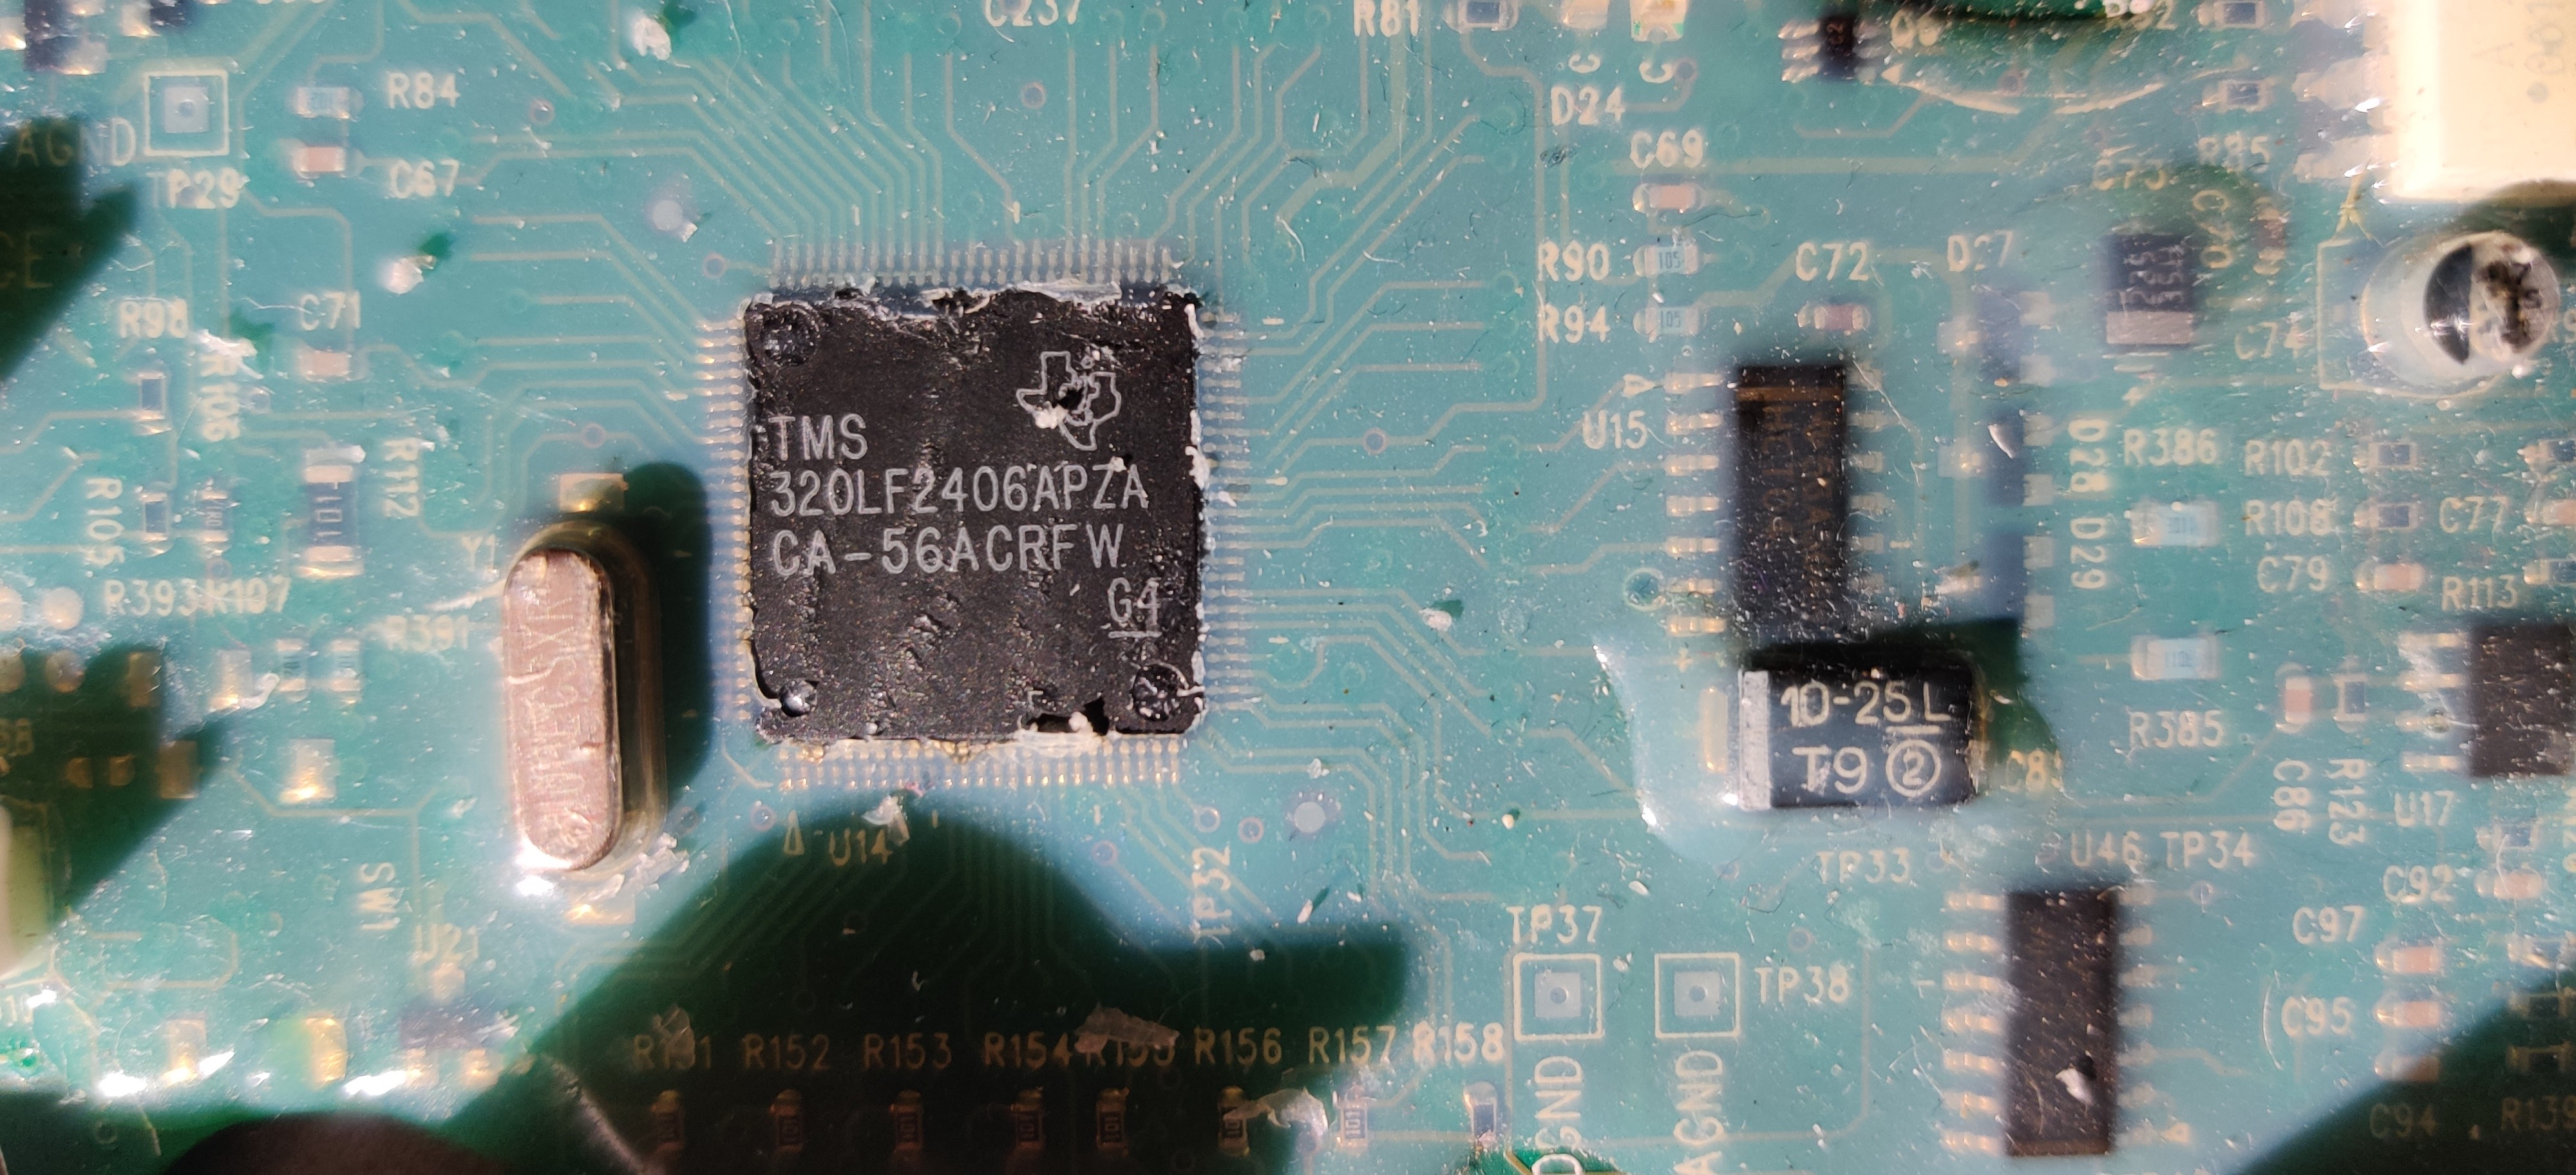
\includegraphics[]{chipImg-320LF2406APZA.jpg}
    \caption{Close-up of a Primary Control Unit DSP (\ref{Component25}) and it's respective traces covered in Conformal Coating}
    \label{fig:chipImg-320LF2406APZA.jpg}
\end{figure}

\subsection{Annotated PCB Images}

\begin{figure}
    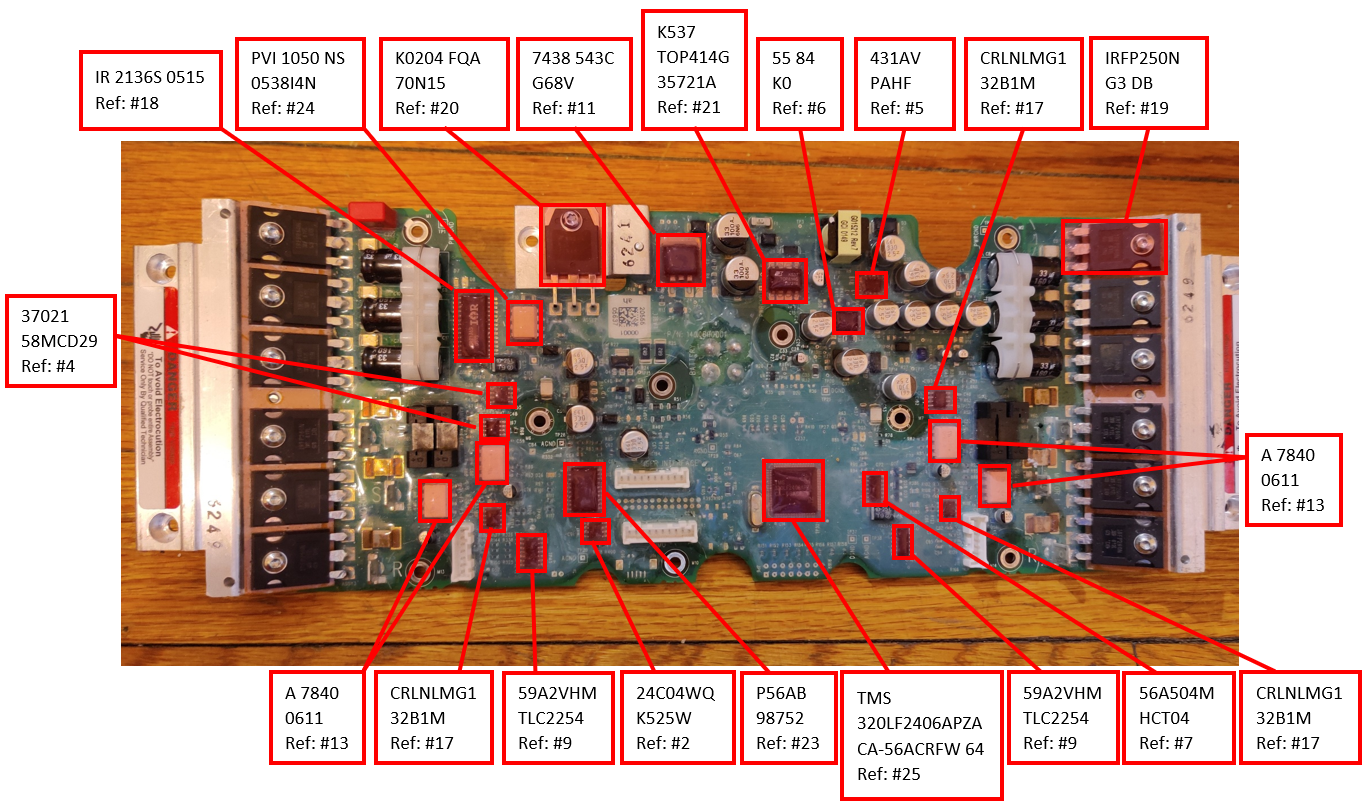
\includegraphics[]{annotatedBoardFront.png}
    \caption{Chip Annotations for the front of a Primary Control Unit}
    \label{fig:annotatedBoardFront.png}
\end{figure}

\begin{figure}
    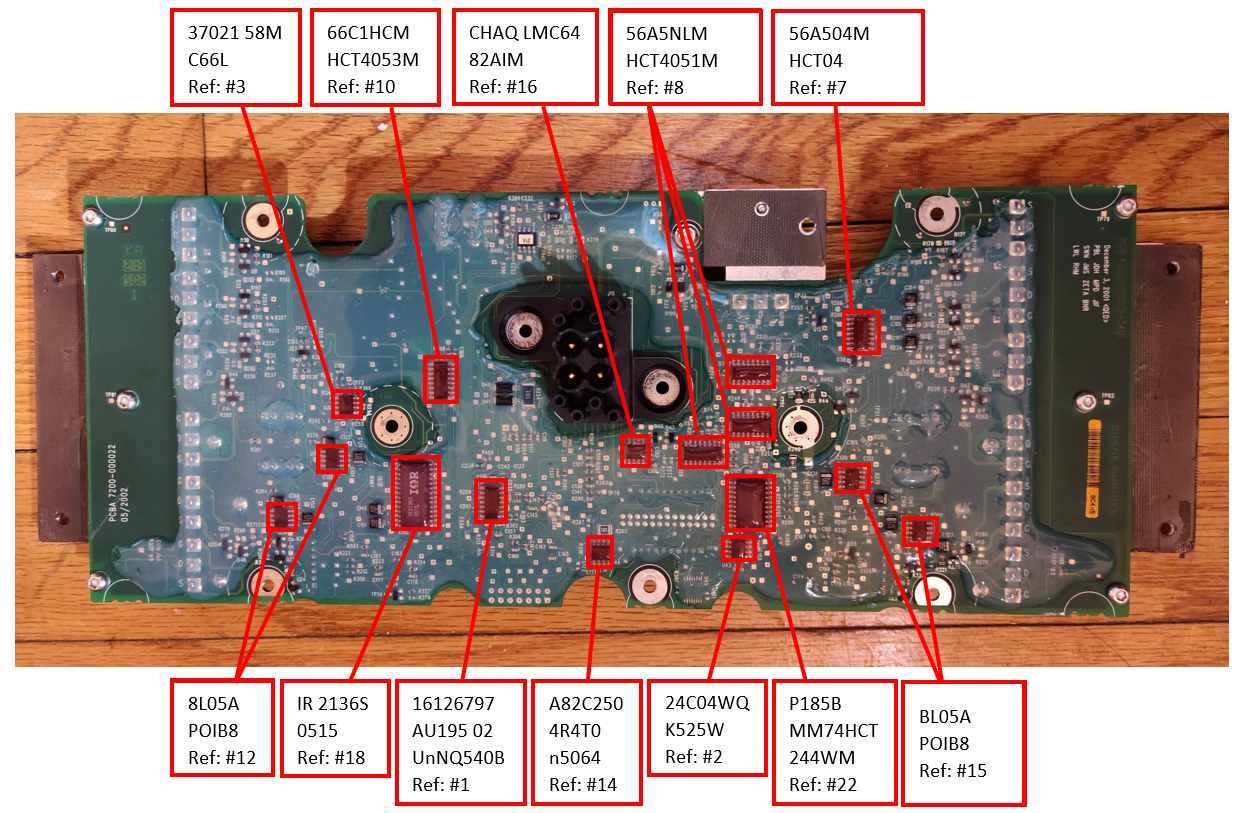
\includegraphics[]{annotatedBoardBack.png}
    \caption{Chip Annotations for the back of a Primary Control Unit}
    \label{fig:annotatedBoardBack.png}
\end{figure}

\begin{figure}
    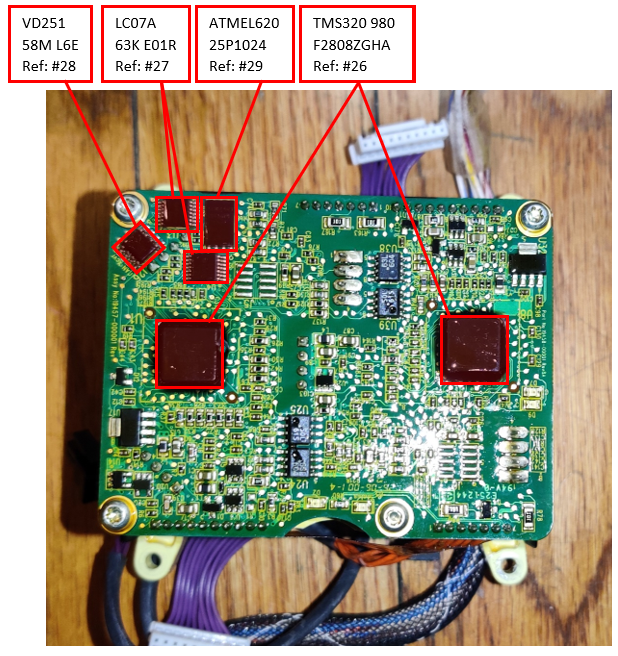
\includegraphics[]{annotatedGyroCubeBottom.png}
    \caption{Annotated view of the main Sensing Unit PCB, with focus on the primary IC components}
    \label{fig:annotatedGyroCubeBottom.jpg}
\end{figure}

\section{Findings}
Focusing on two of the most important components:
\begin{itemize}
    \item Sensing Unit (SU)
    \item Primary Control Unit (PCU)
\end{itemize}

\subsection{Sensing Unit}
The sensor unit is located in the center of the Segway and consists of 5 simple IMU sensors. Referencing Figure \ref{fig:segwayGyroCubeBottom.jpg}, the shared PCB between the IMUs contains two TI TMS320980 DSP (\ref{Component26}), a TI VD251 CAN Bus Transceiver (\ref{Component28}), and an ATMEL SPI Interface (\ref{Component29}), plus two TI LV07A Hex Buffers (\ref{Component27}). The TI DSP components provide data fusion between the IMUs, in close proximity to protect from motor-generated noise. We believe the presence of two DSP components both serves for redundancy, and to allocate one DSP to supply fused sensor data to each PCU.

As shown in (\ref{fig:segwayGyroCubeTop.jpg}), each IMU is in a different orientation to account for \href{https://base.xsens.com/hc/en-us/articles/209611089-Understanding-Sensor-Bias-offset-}{sensor-specific bias instability and angular random walk}, allowing for a partial mechanical cancellation of various biases present in the sensors. 

This board utilizes both SPI and CAN. We assume utilizing the high-speed SPI interface to send fused orientation data to the PCU (master) and CAN connecting all major components for system-specific diagnostics relayed to the Segway handheld control.

\subsection{Primary Control Unit}
The PCU contains most of the Segway’s components and handles motor control. The Segway contains two identical PCUs, each connecting directly to each three-phase motor, as shown in [REF MOTOR PLUGS]. Being three-phase with a six-phase input, we believe this to be for redundancy, or for mirrored motor driving. The PCU contains a TI TMS320LF240 DSP. This DSP likely manages the battery system (managed by three demultiplexers - \ref{Component8}) which utilizes \href{https://github.com/martinbogo/pt-battery-diagnostics}{I2C communications} for battery state/management. We assume the DSP also handles motor position/rotation data, current sensing data, and orientation data from the sensing unit to perform adjustments during travel, keeping the rider upright. The DSP has separate program and data memory spaces. This not only allows for simultaneous instruction fetch and execution but also for simultaneous transfers between memory spaces. This removes the need to interrupt the process flow to fetch external instructions (such as reading from sensor SPI data), allowing the component to perform without halting and performing at full speed.

\section{Conclusion}
There is so much we couldn’t detail here. We learned so much about the intricacies of a complicated real-time system, intuitive sensor shielding and processing, and how the Segway becomes a “smart device” through I2C, SPI, and CAN communications between modules for system health checks and data transfer.

\section{Disassembly Figures}

\subsection{Segway Exterior}

\begin{figure}
    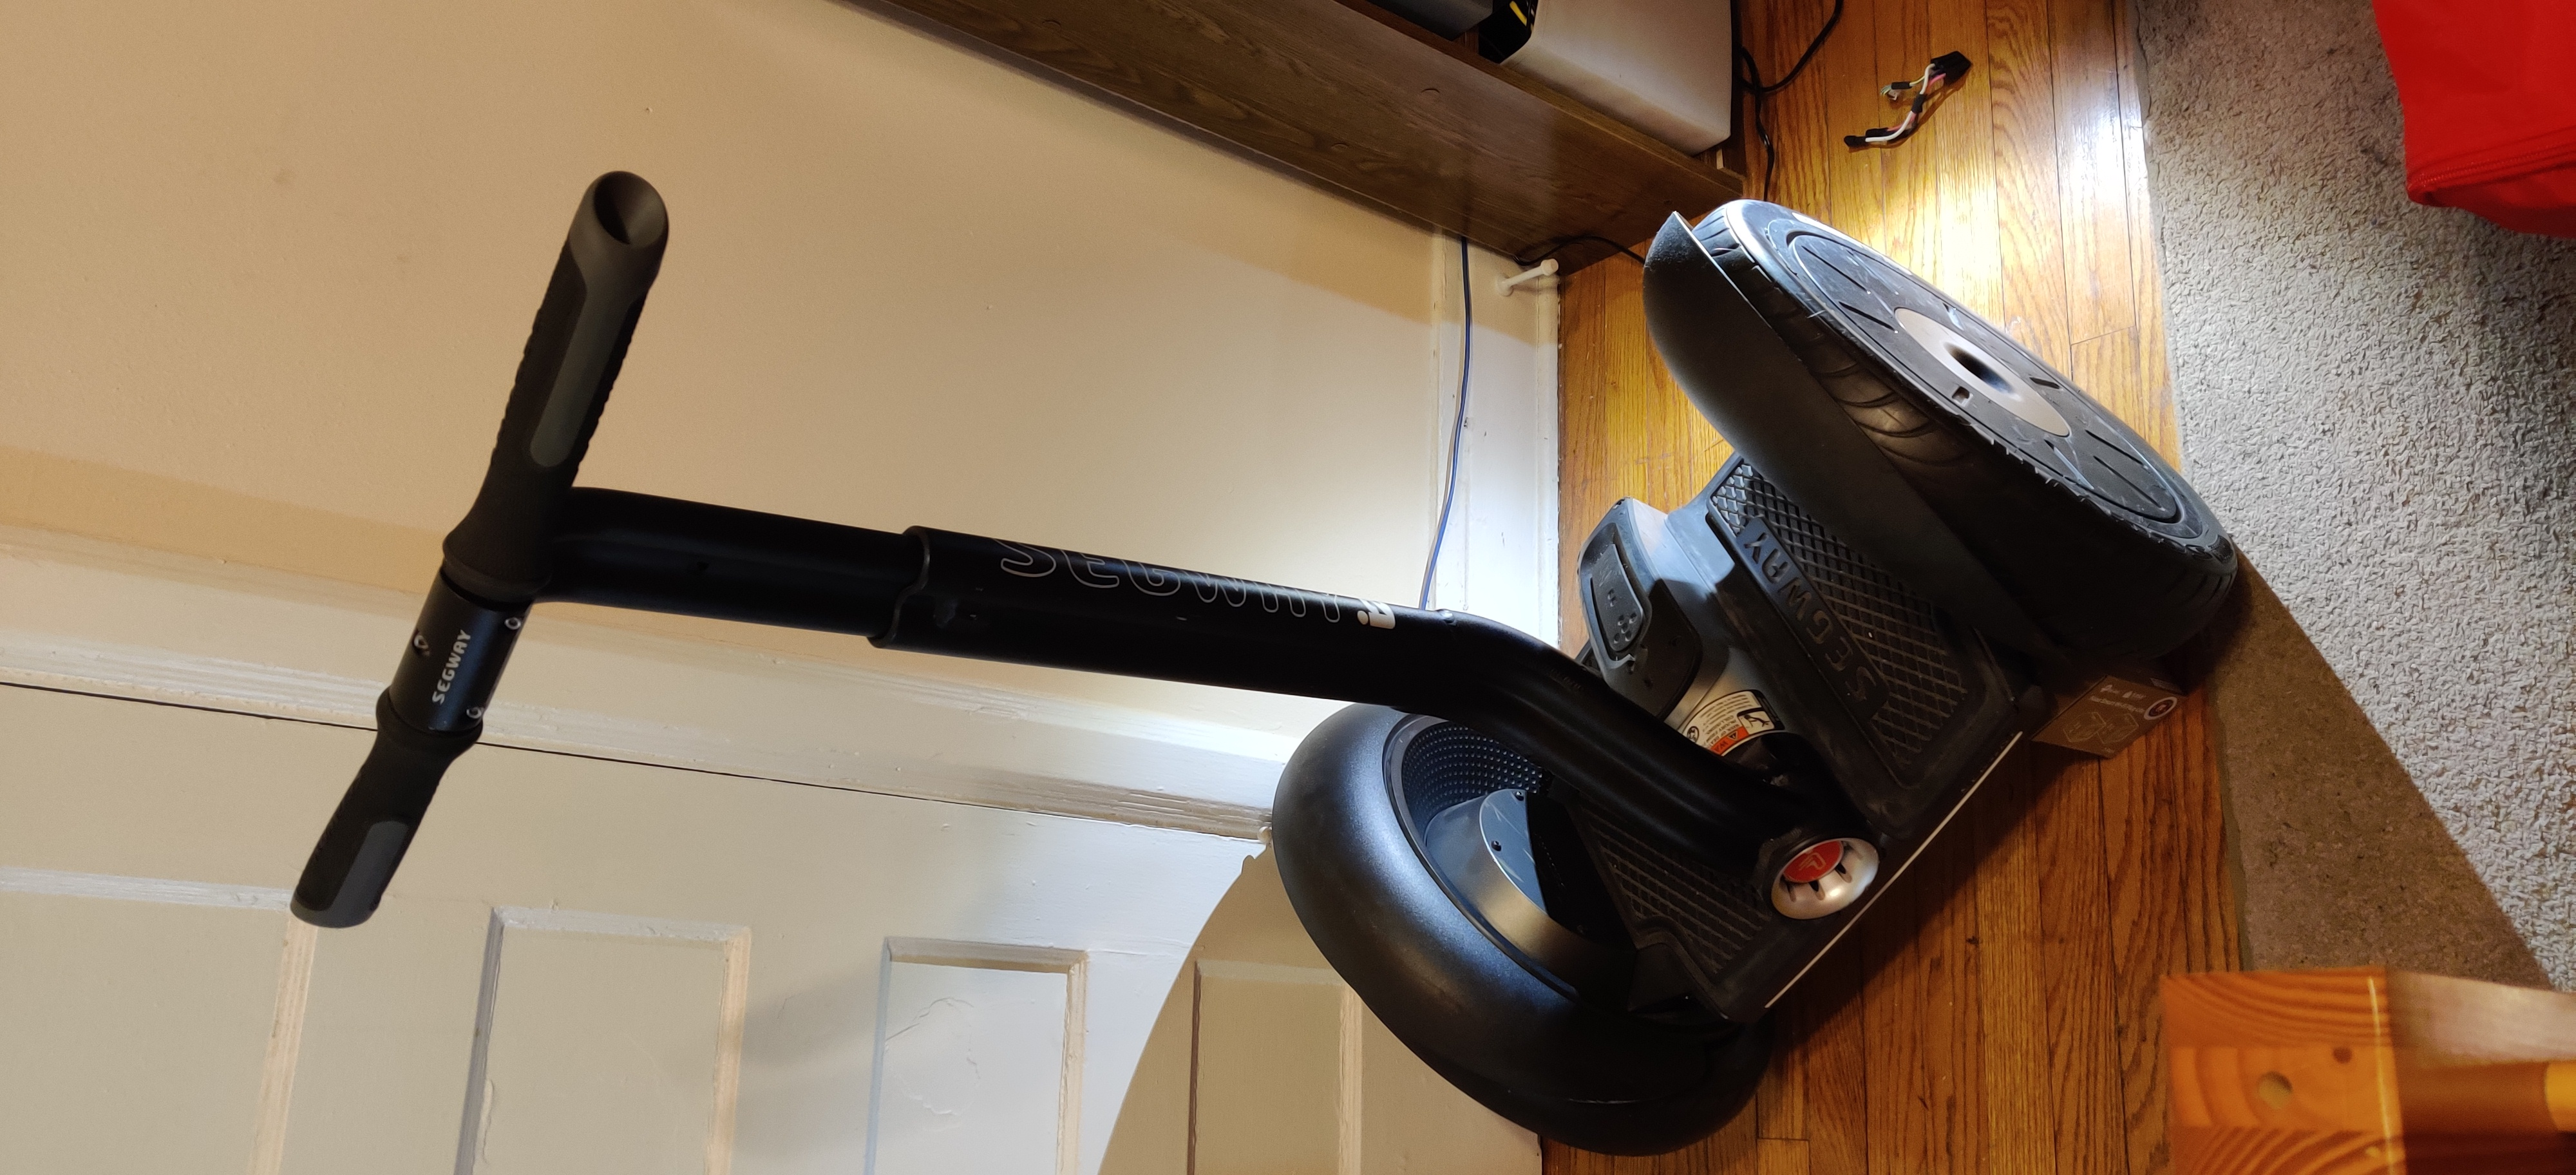
\includegraphics[angle=-90]{segwayFront.jpg}
    \caption{Front view of the assembled Segway, including all trim pieces}
    \label{fig:segwayFront.jpg}
\end{figure}

\begin{figure}
    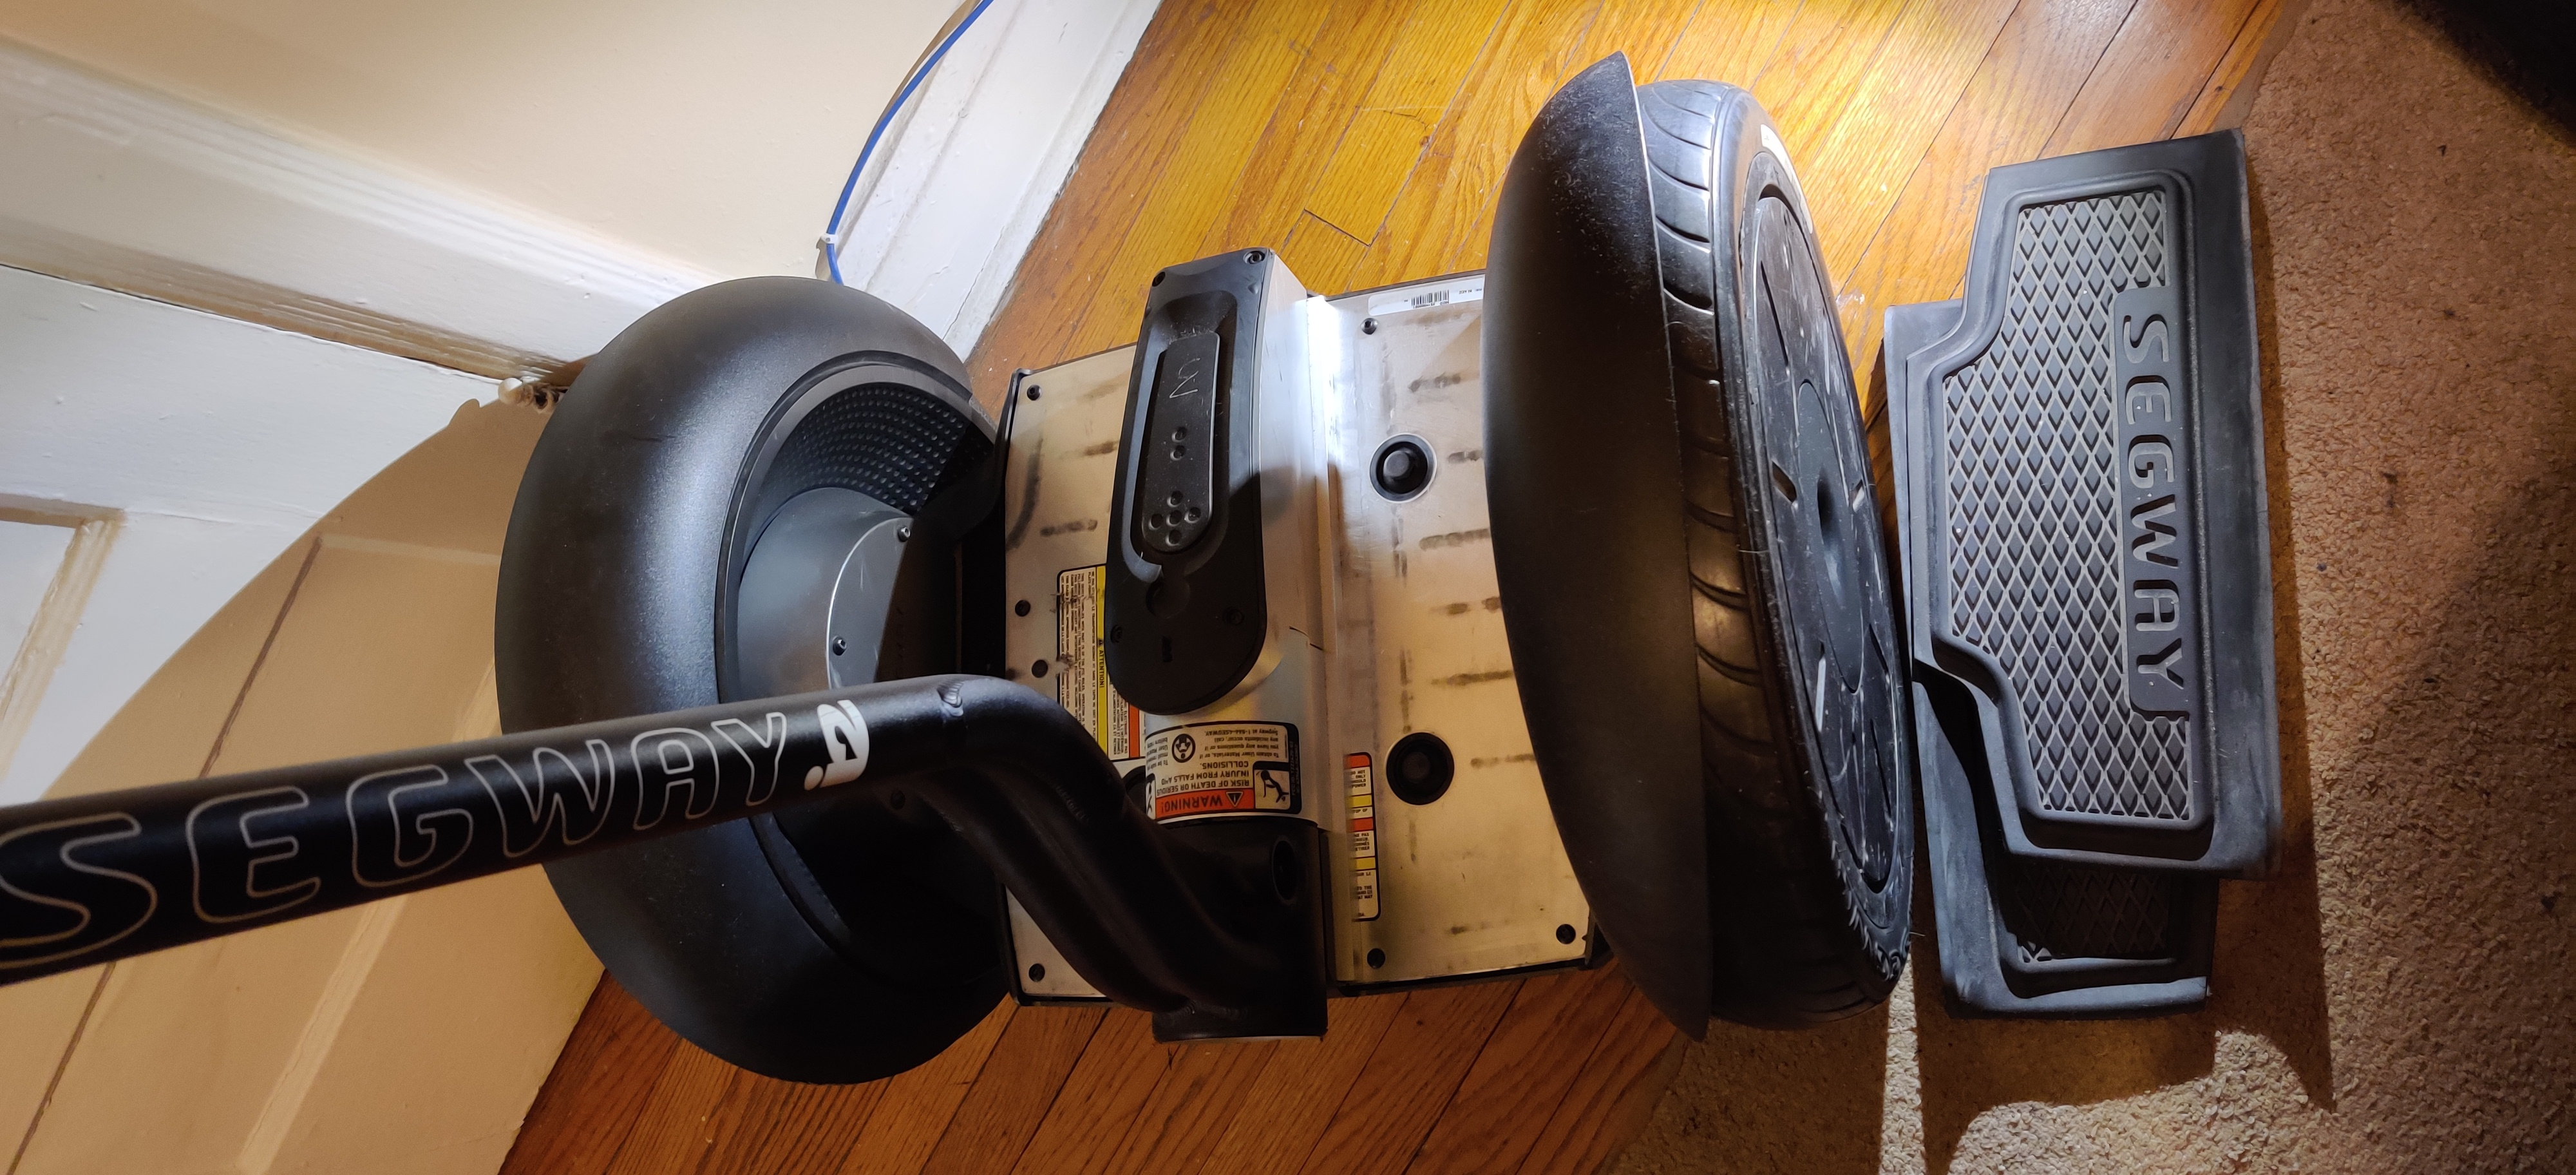
\includegraphics[angle=-90]{segwayPadsRemoved.jpg}
    \caption{Segway platform with rubber trim pieces removed}
    \label{fig:segwayPadsRemoved.jpg}
\end{figure}

\begin{figure}
    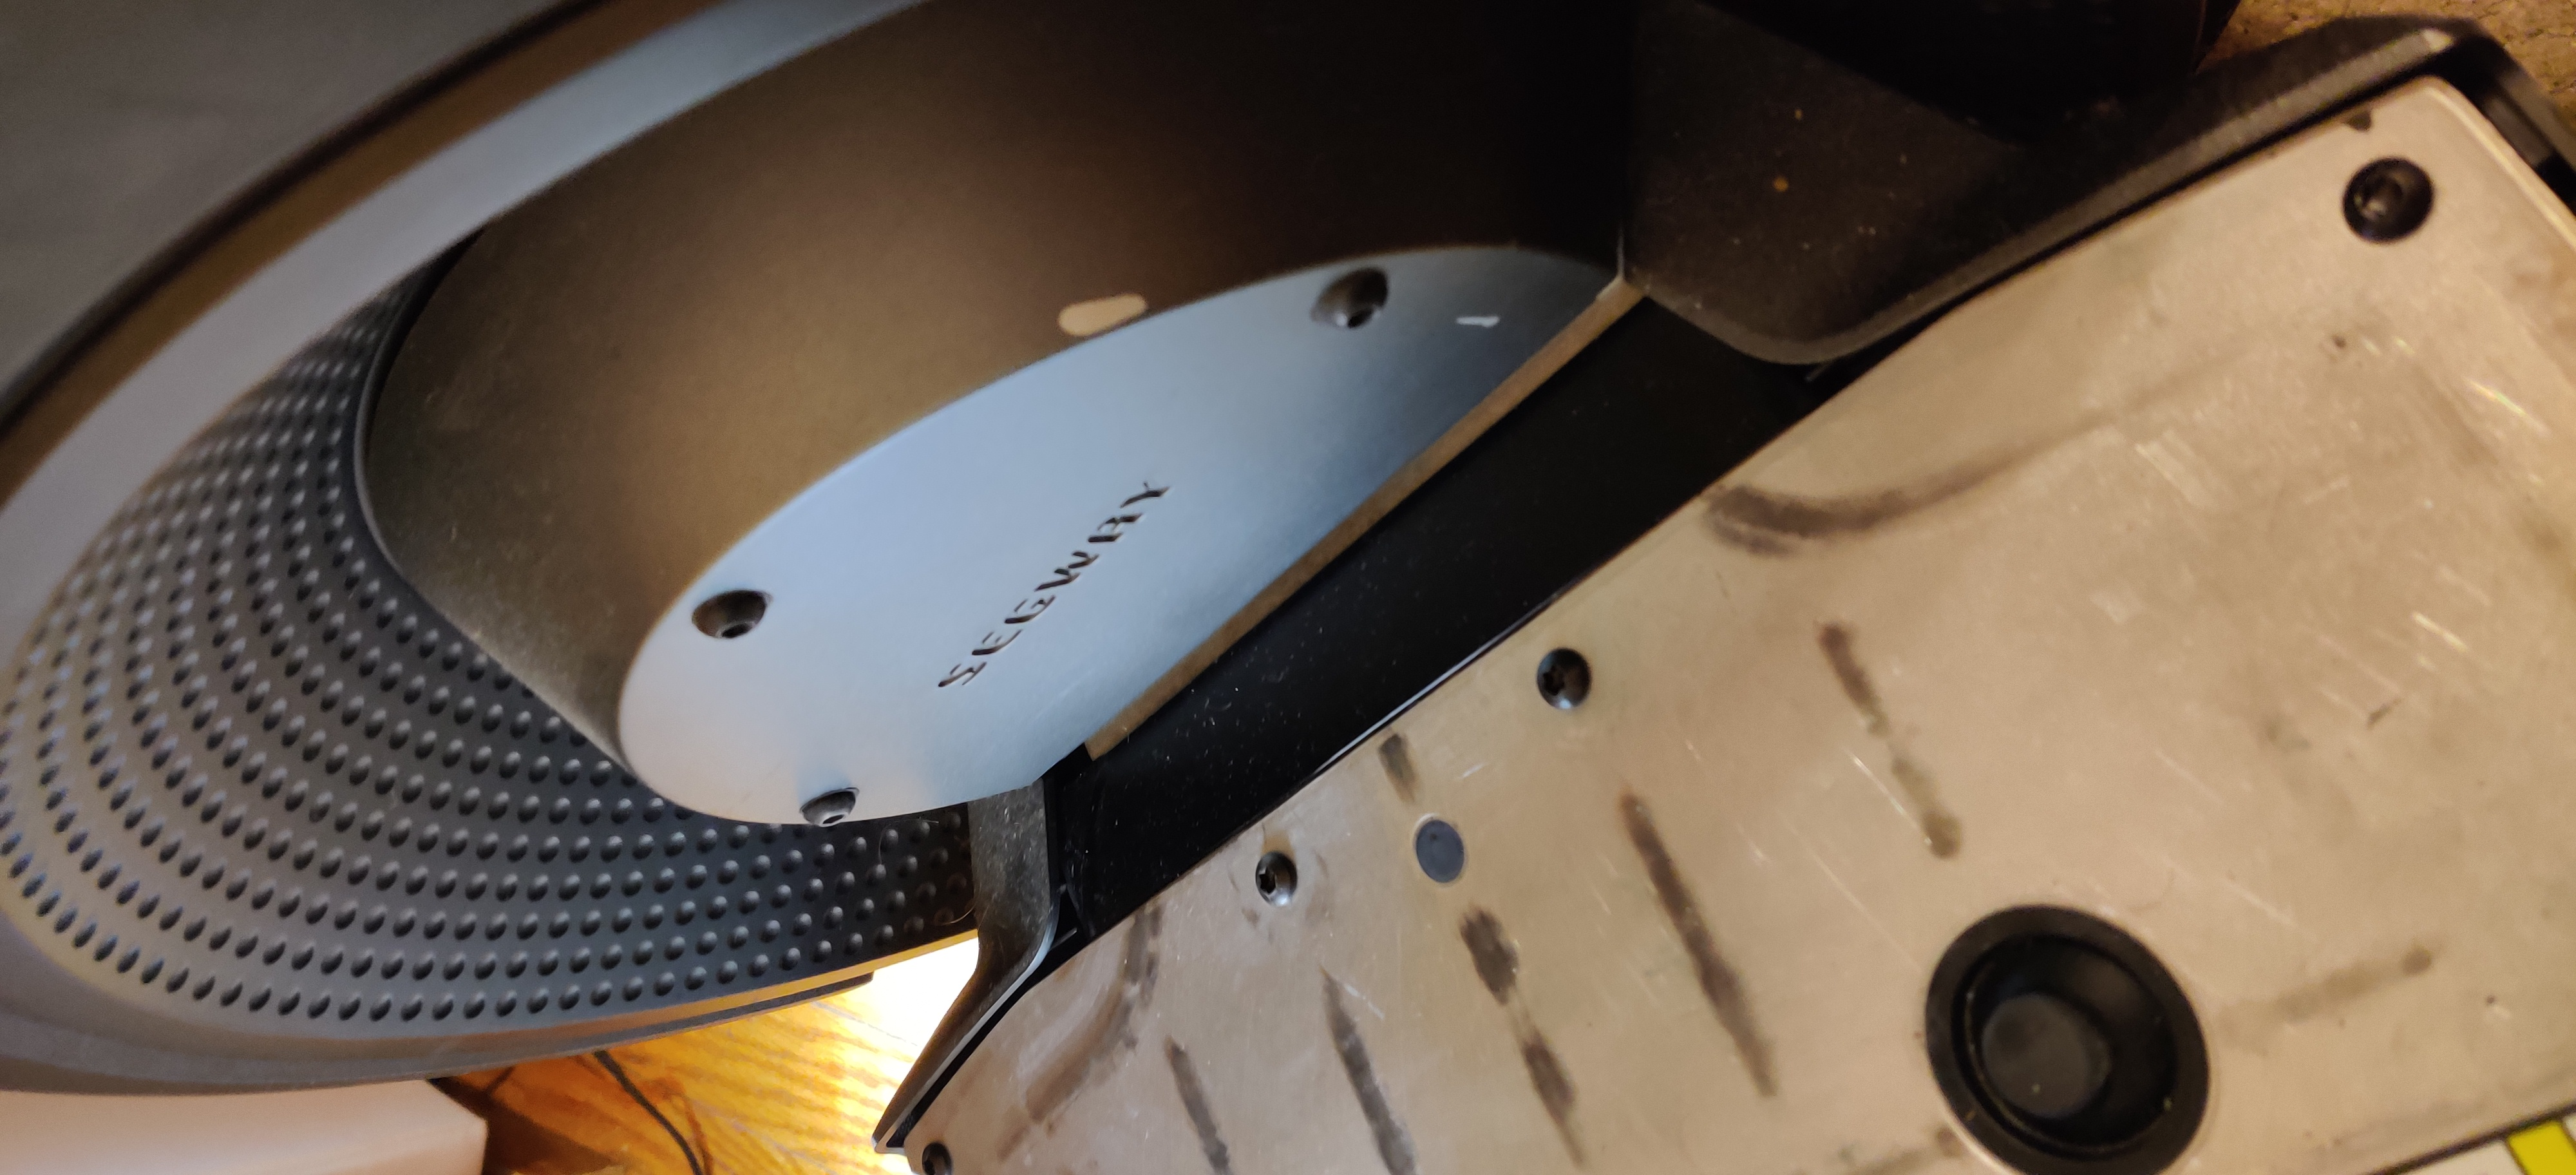
\includegraphics[angle=-90]{segwayWheelAttachment.jpg}
    \caption{Side wheel trim piece firmly mounted to the platform}
    \label{fig:segwayWheelAttachment.jpg}
\end{figure}

\begin{figure}
    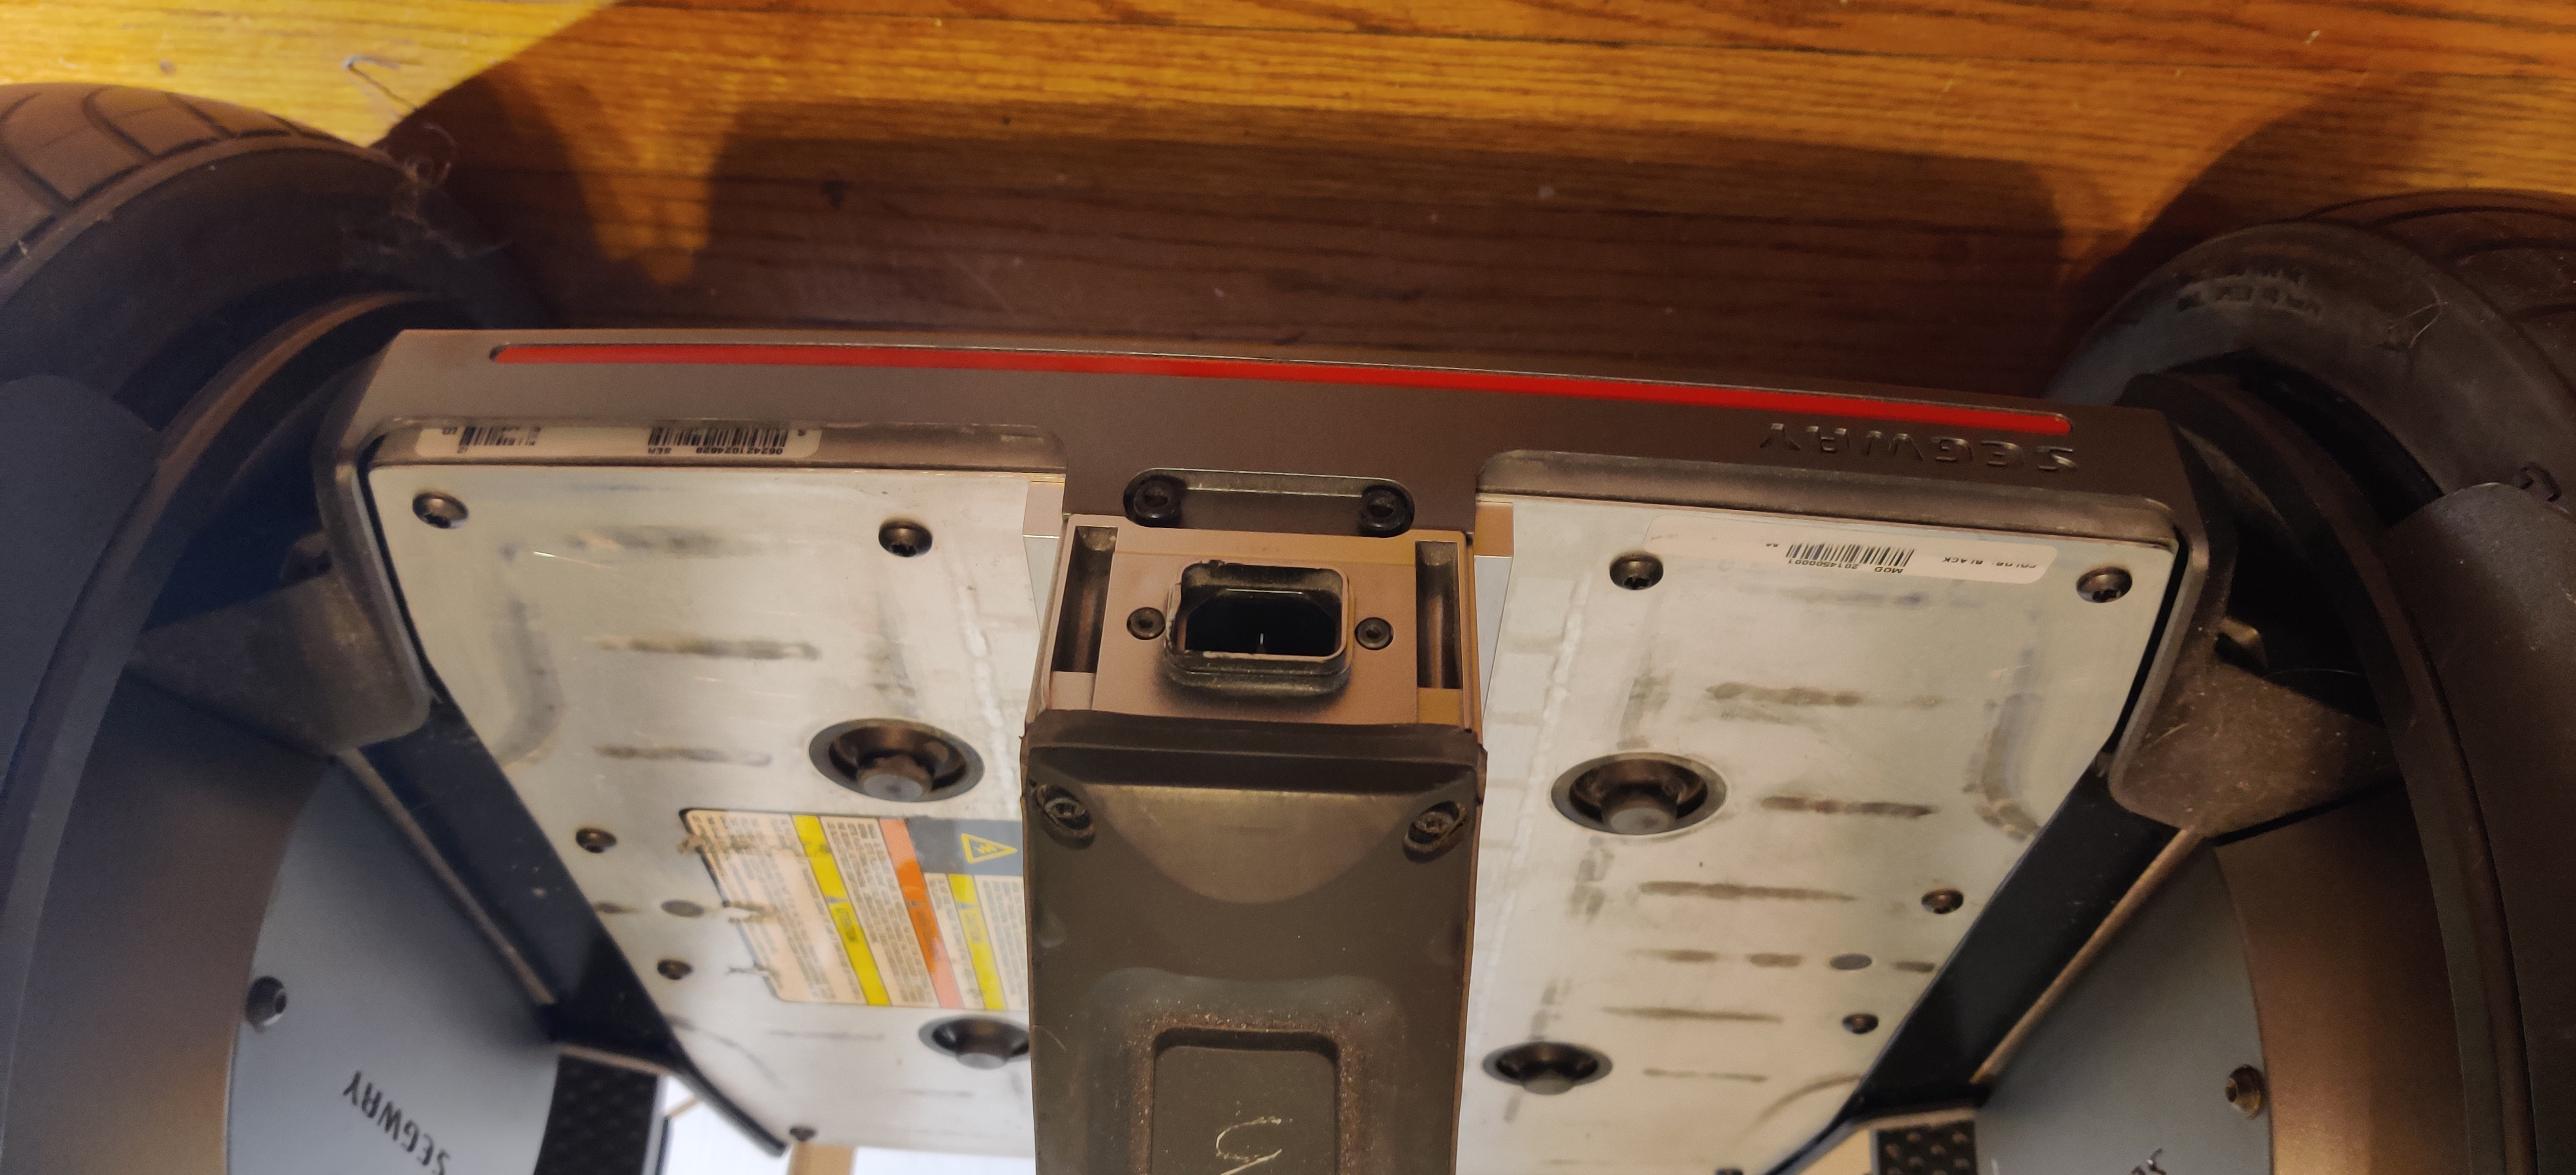
\includegraphics[angle=180]{segwayRear.jpg}
    \caption{Segway charging port (rear) with rubber trim pieces removed}
    \label{fig:segwayRear.jpg}
\end{figure}

\begin{figure}
    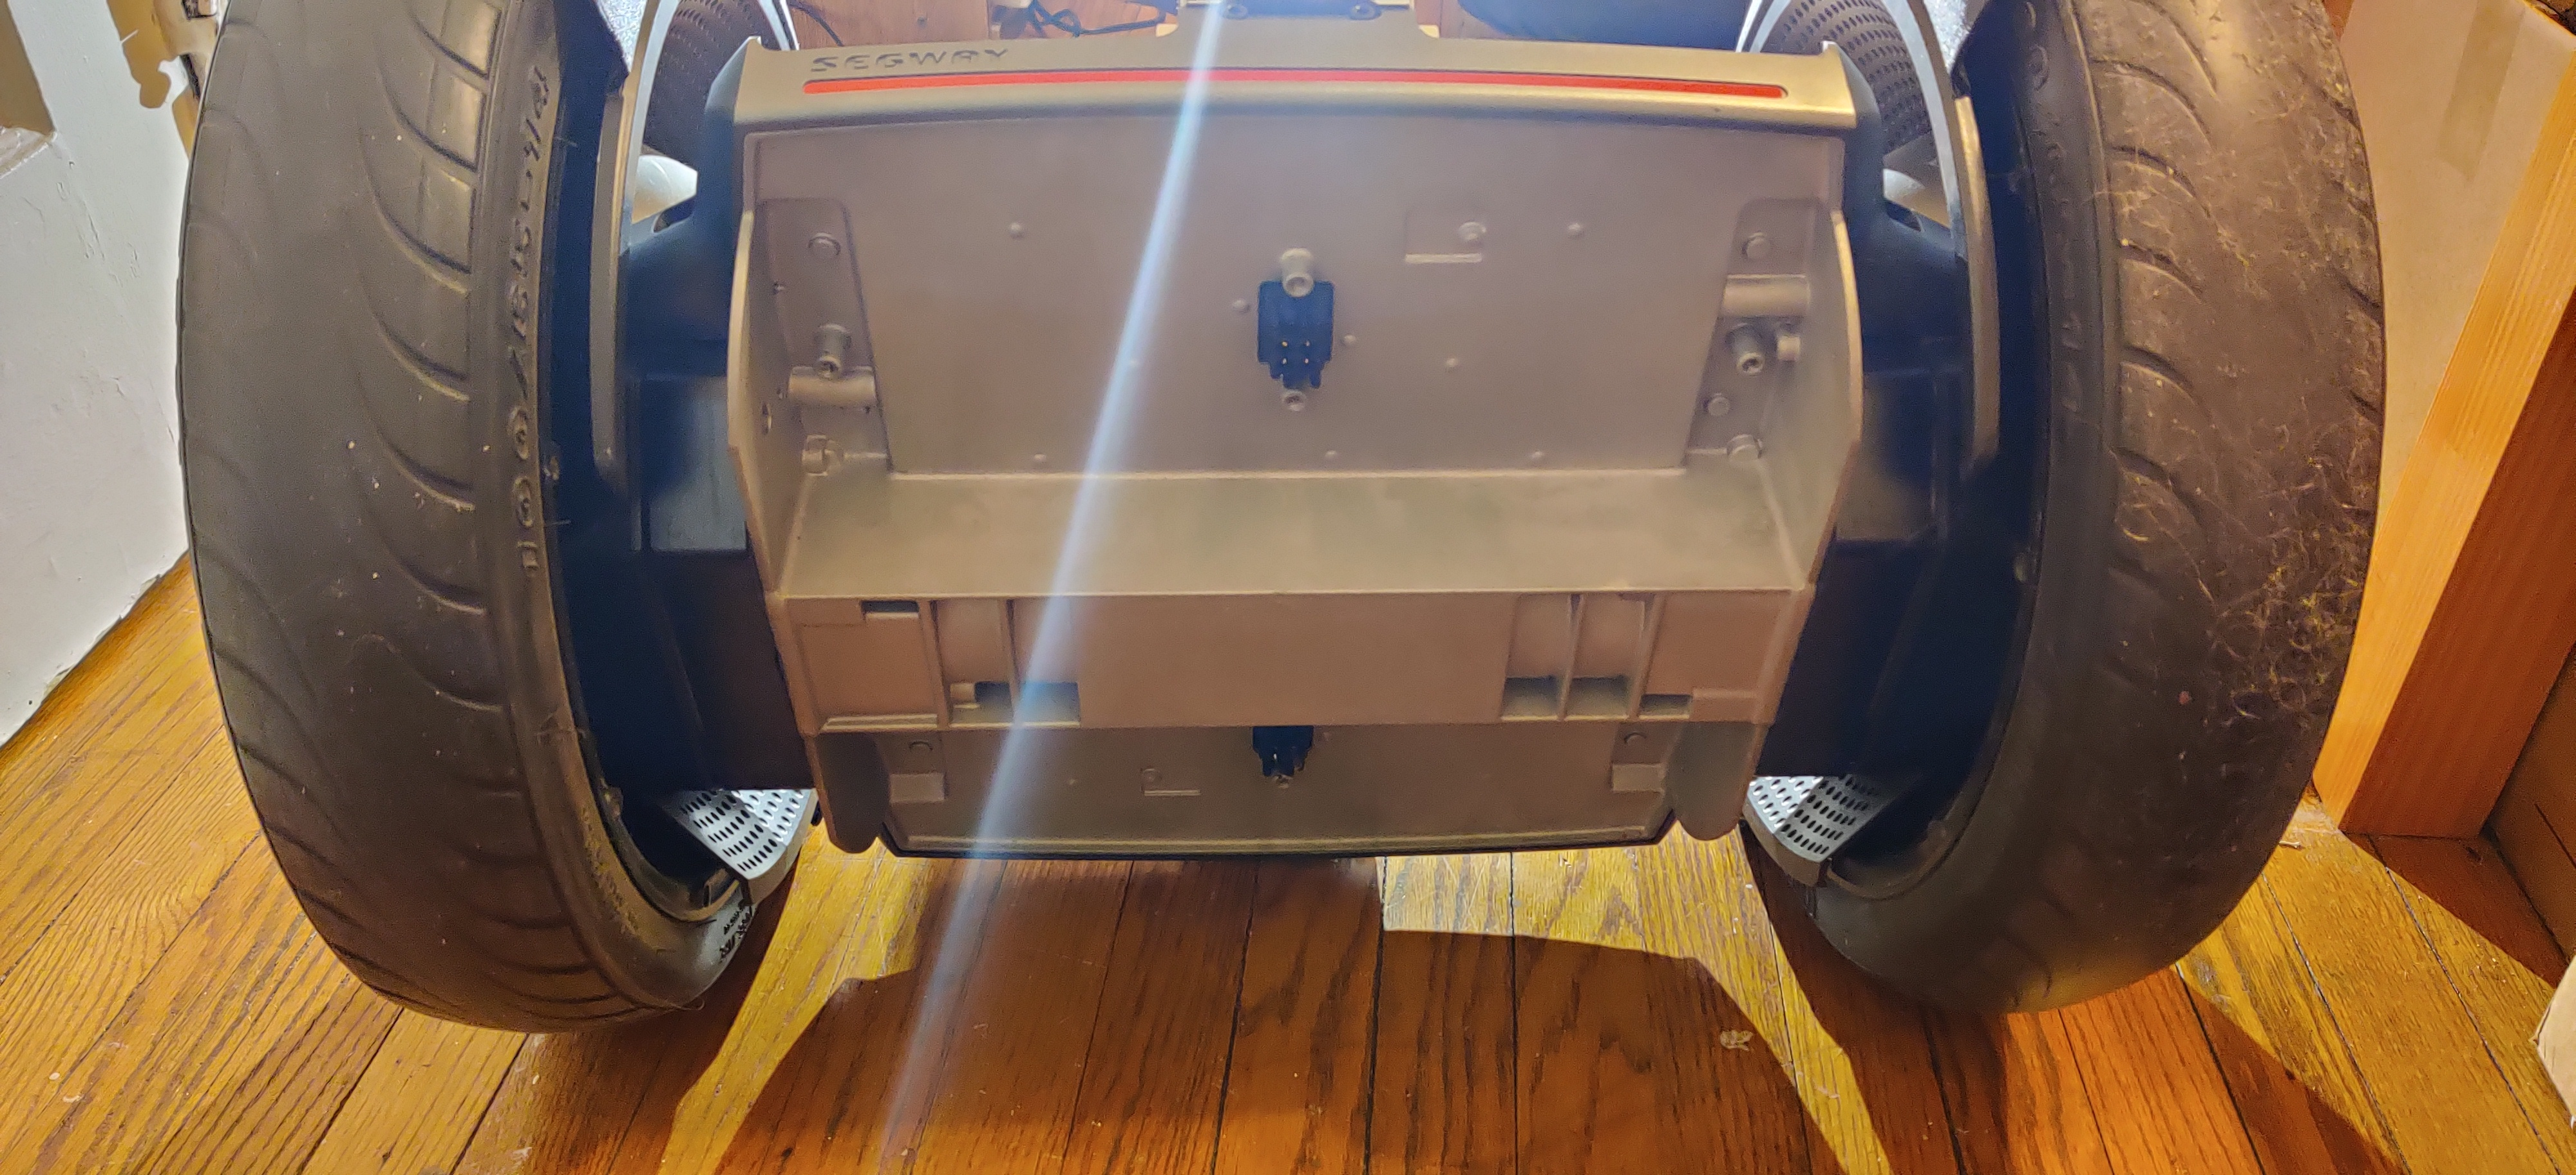
\includegraphics[]{segwayBottom.jpg}
    \caption{Dual Steel Battery Bays for the Segway. Each battery connector supports ~74V connections and I2C communications}
    \label{fig:segwayBottom.jpg}
\end{figure}

\subsection{Segway Interior}

\begin{figure}
    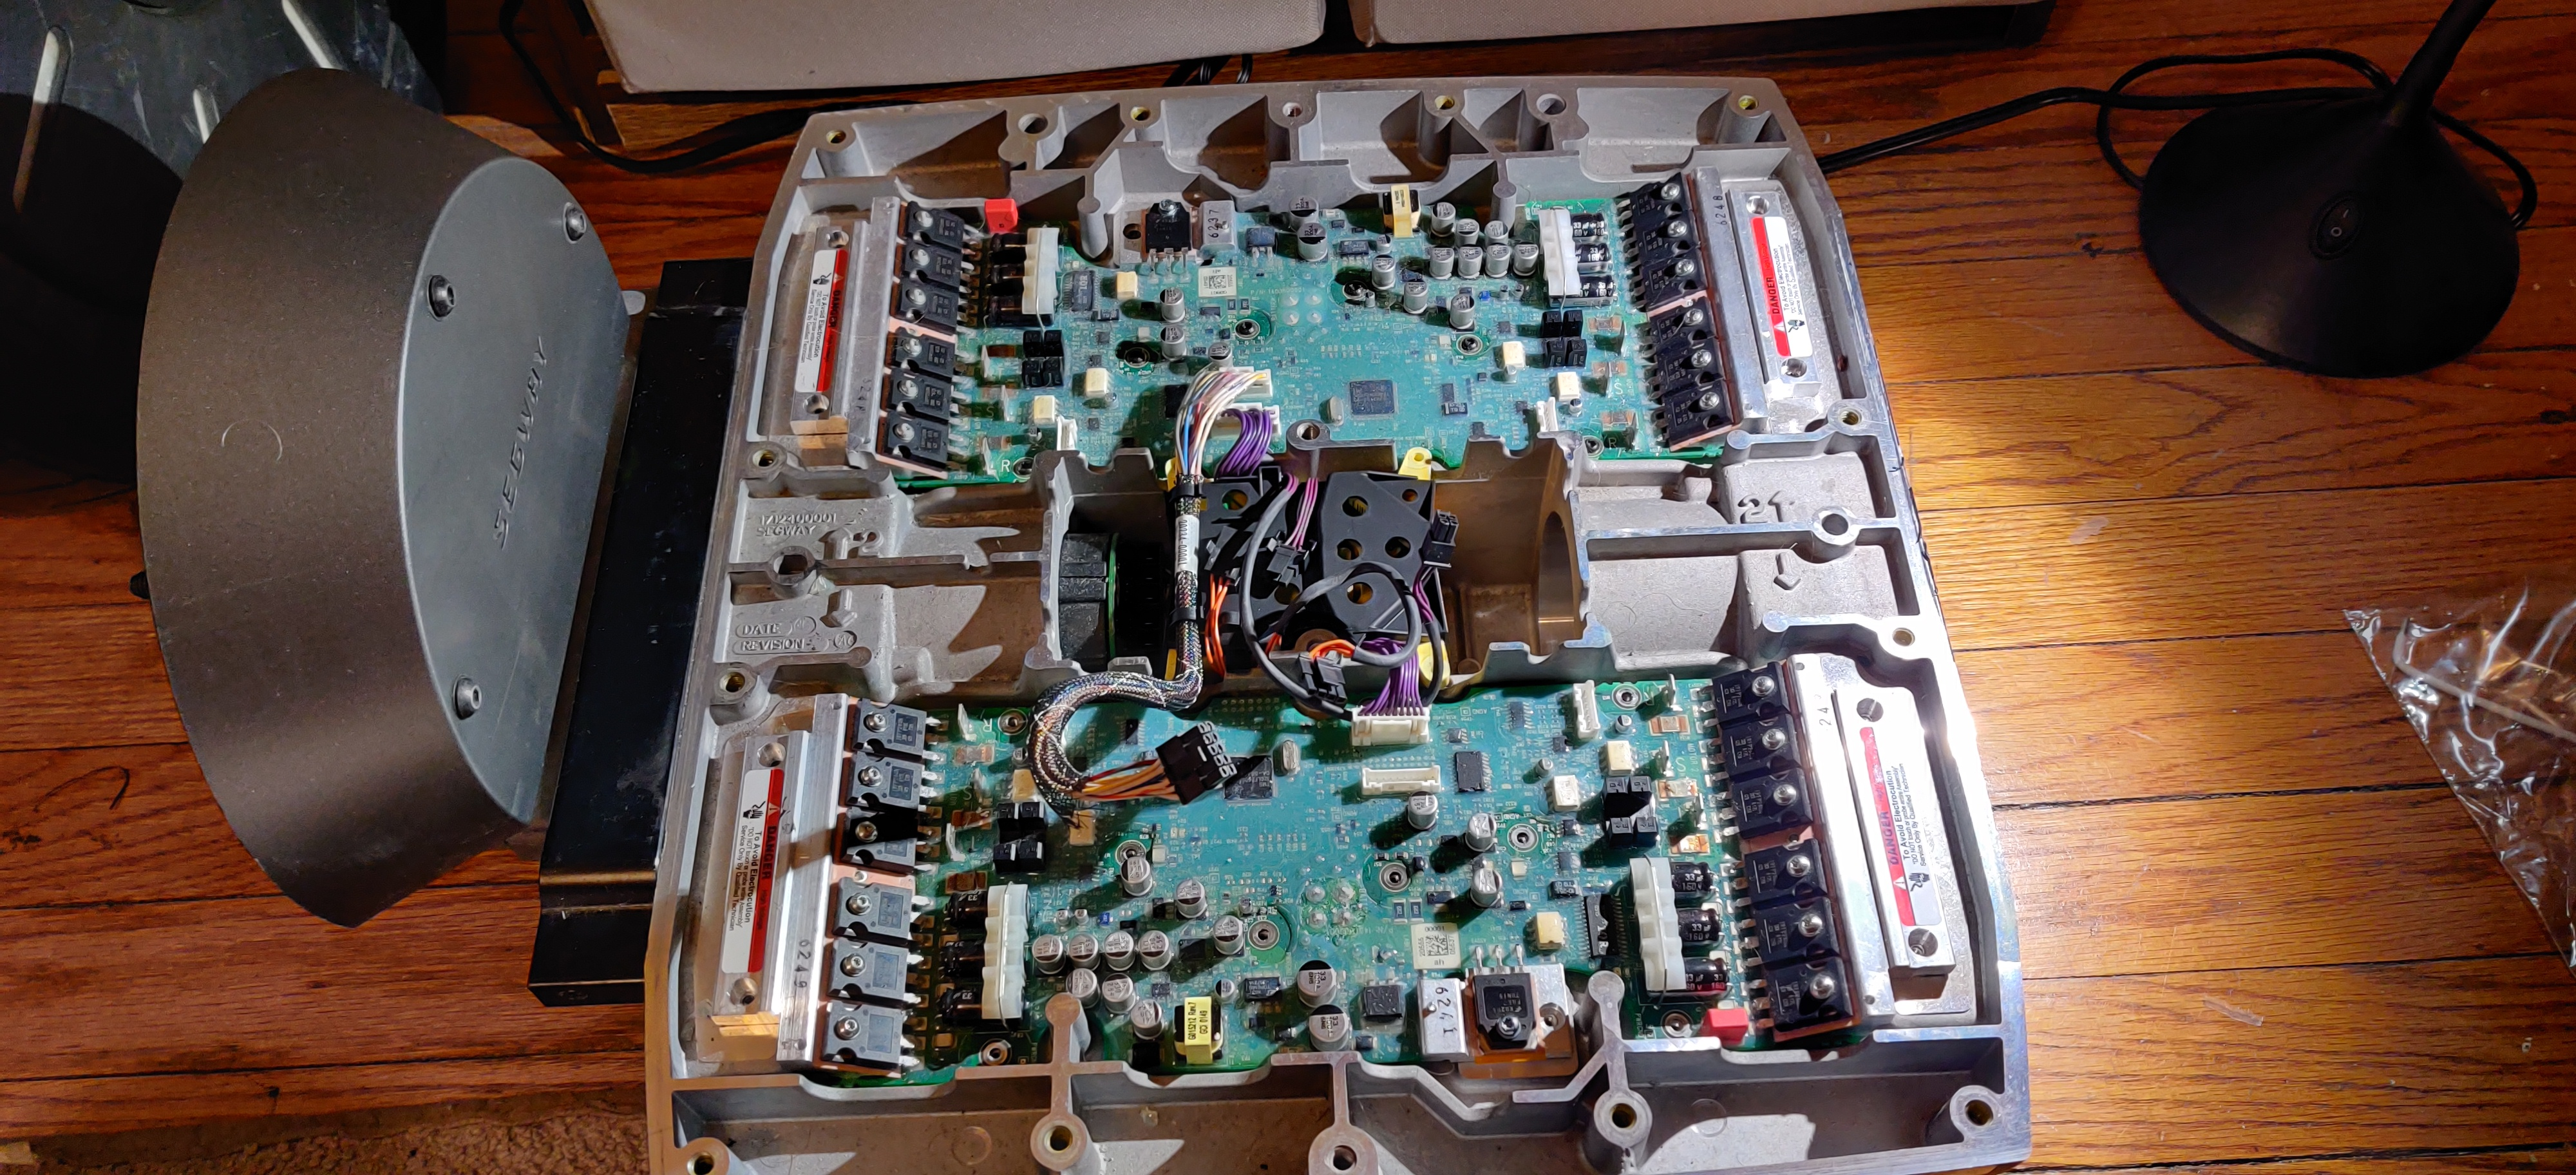
\includegraphics[]{segwayInternalsTop.jpg}
    \caption{Segway Chassis without one wheel well and the platform, which exposes both Primary Control Units and the Sensing Unit in the center}
    \label{fig:segwayInternalsTop.jpg}
\end{figure}

\subsubsection{Primary Control Unit}

\begin{figure}
    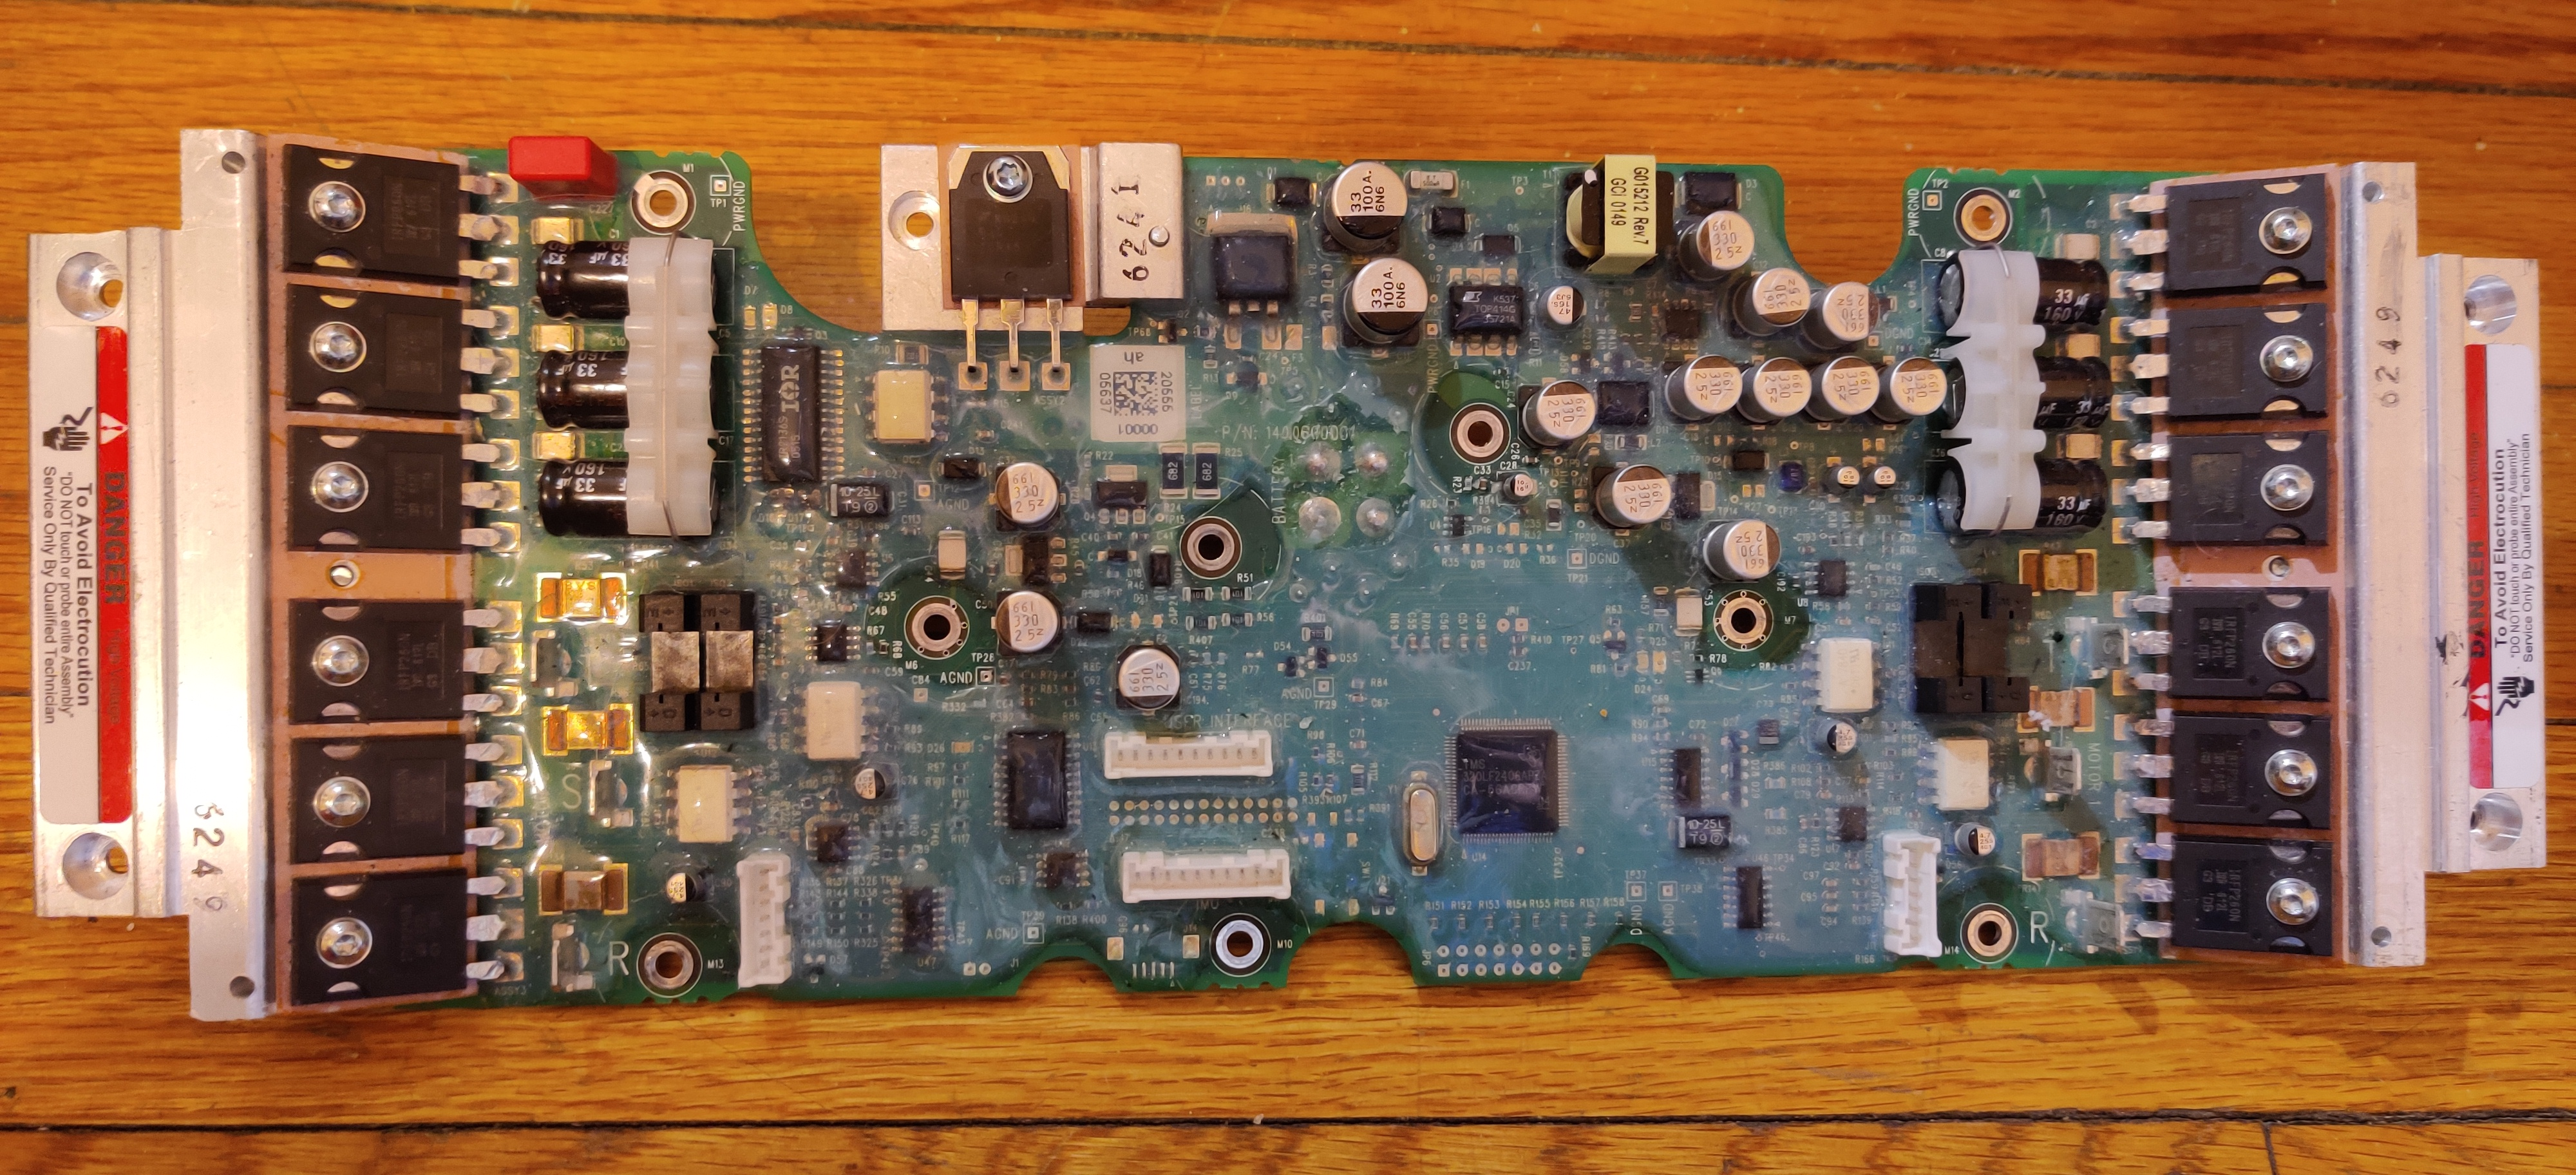
\includegraphics[]{entireBoardTop.jpg}
    \caption{Top of one of the two Primary Control Units, covered in Conformal Coating surrounding the surface mount components}
    \label{fig:entireBoardTop.jpg}
\end{figure}

\begin{figure}
    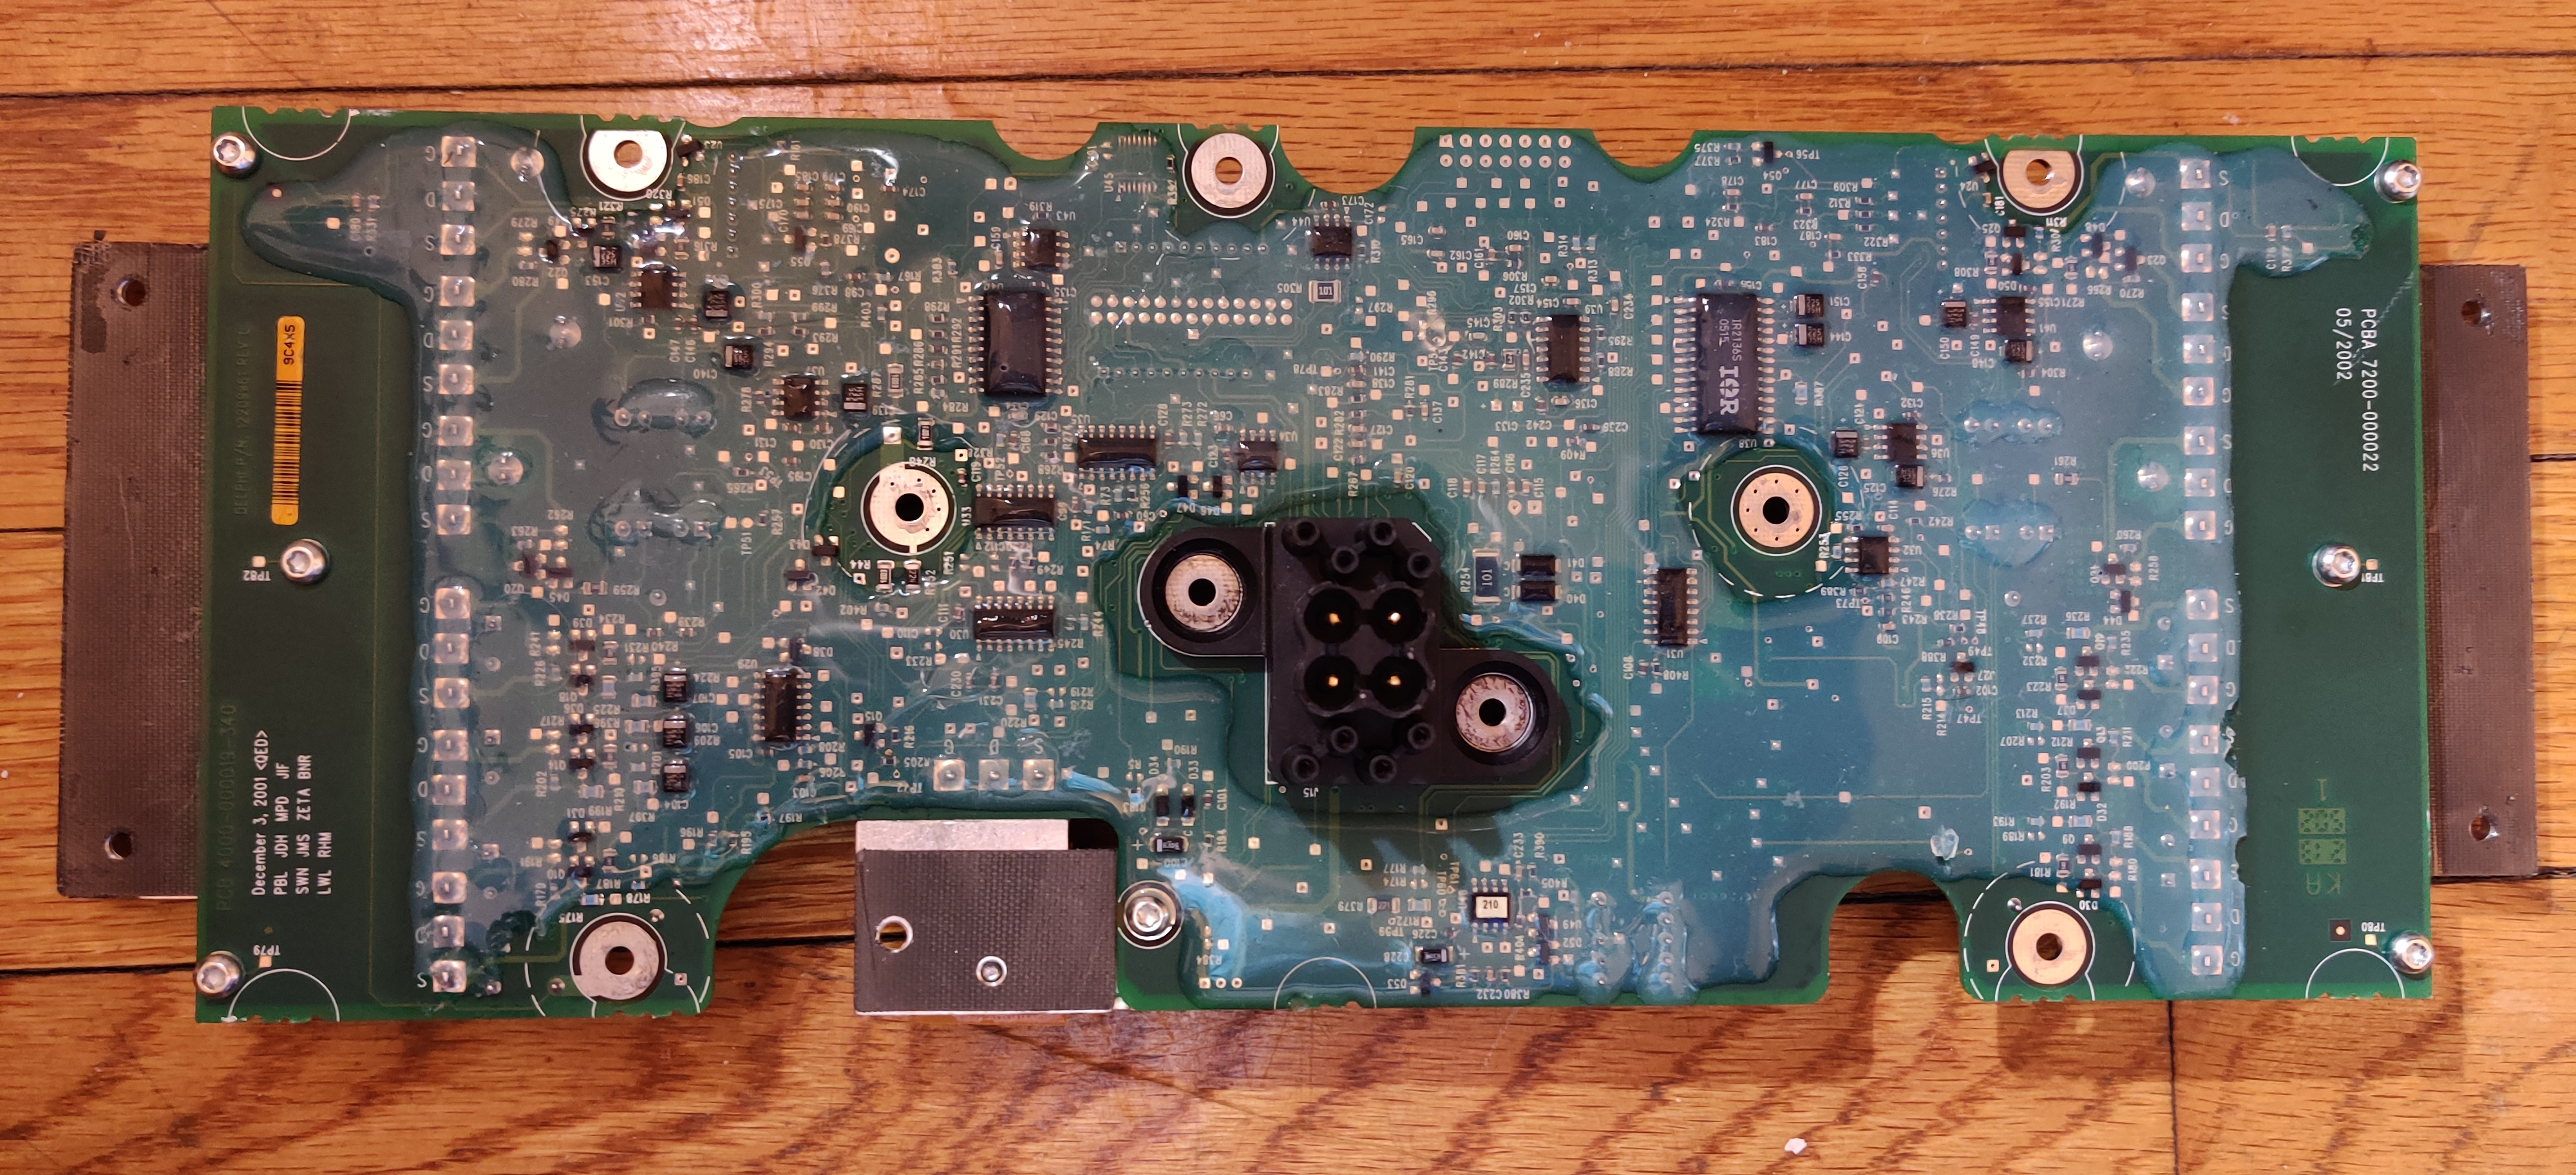
\includegraphics[]{entireBoardBottom.jpg}
    \caption{Bottom of one of the two Primary Control Units, covered in a thick layer of Conformal Coating}
    \label{fig:entireBoardBottom.jpg}
\end{figure}

\begin{figure}
    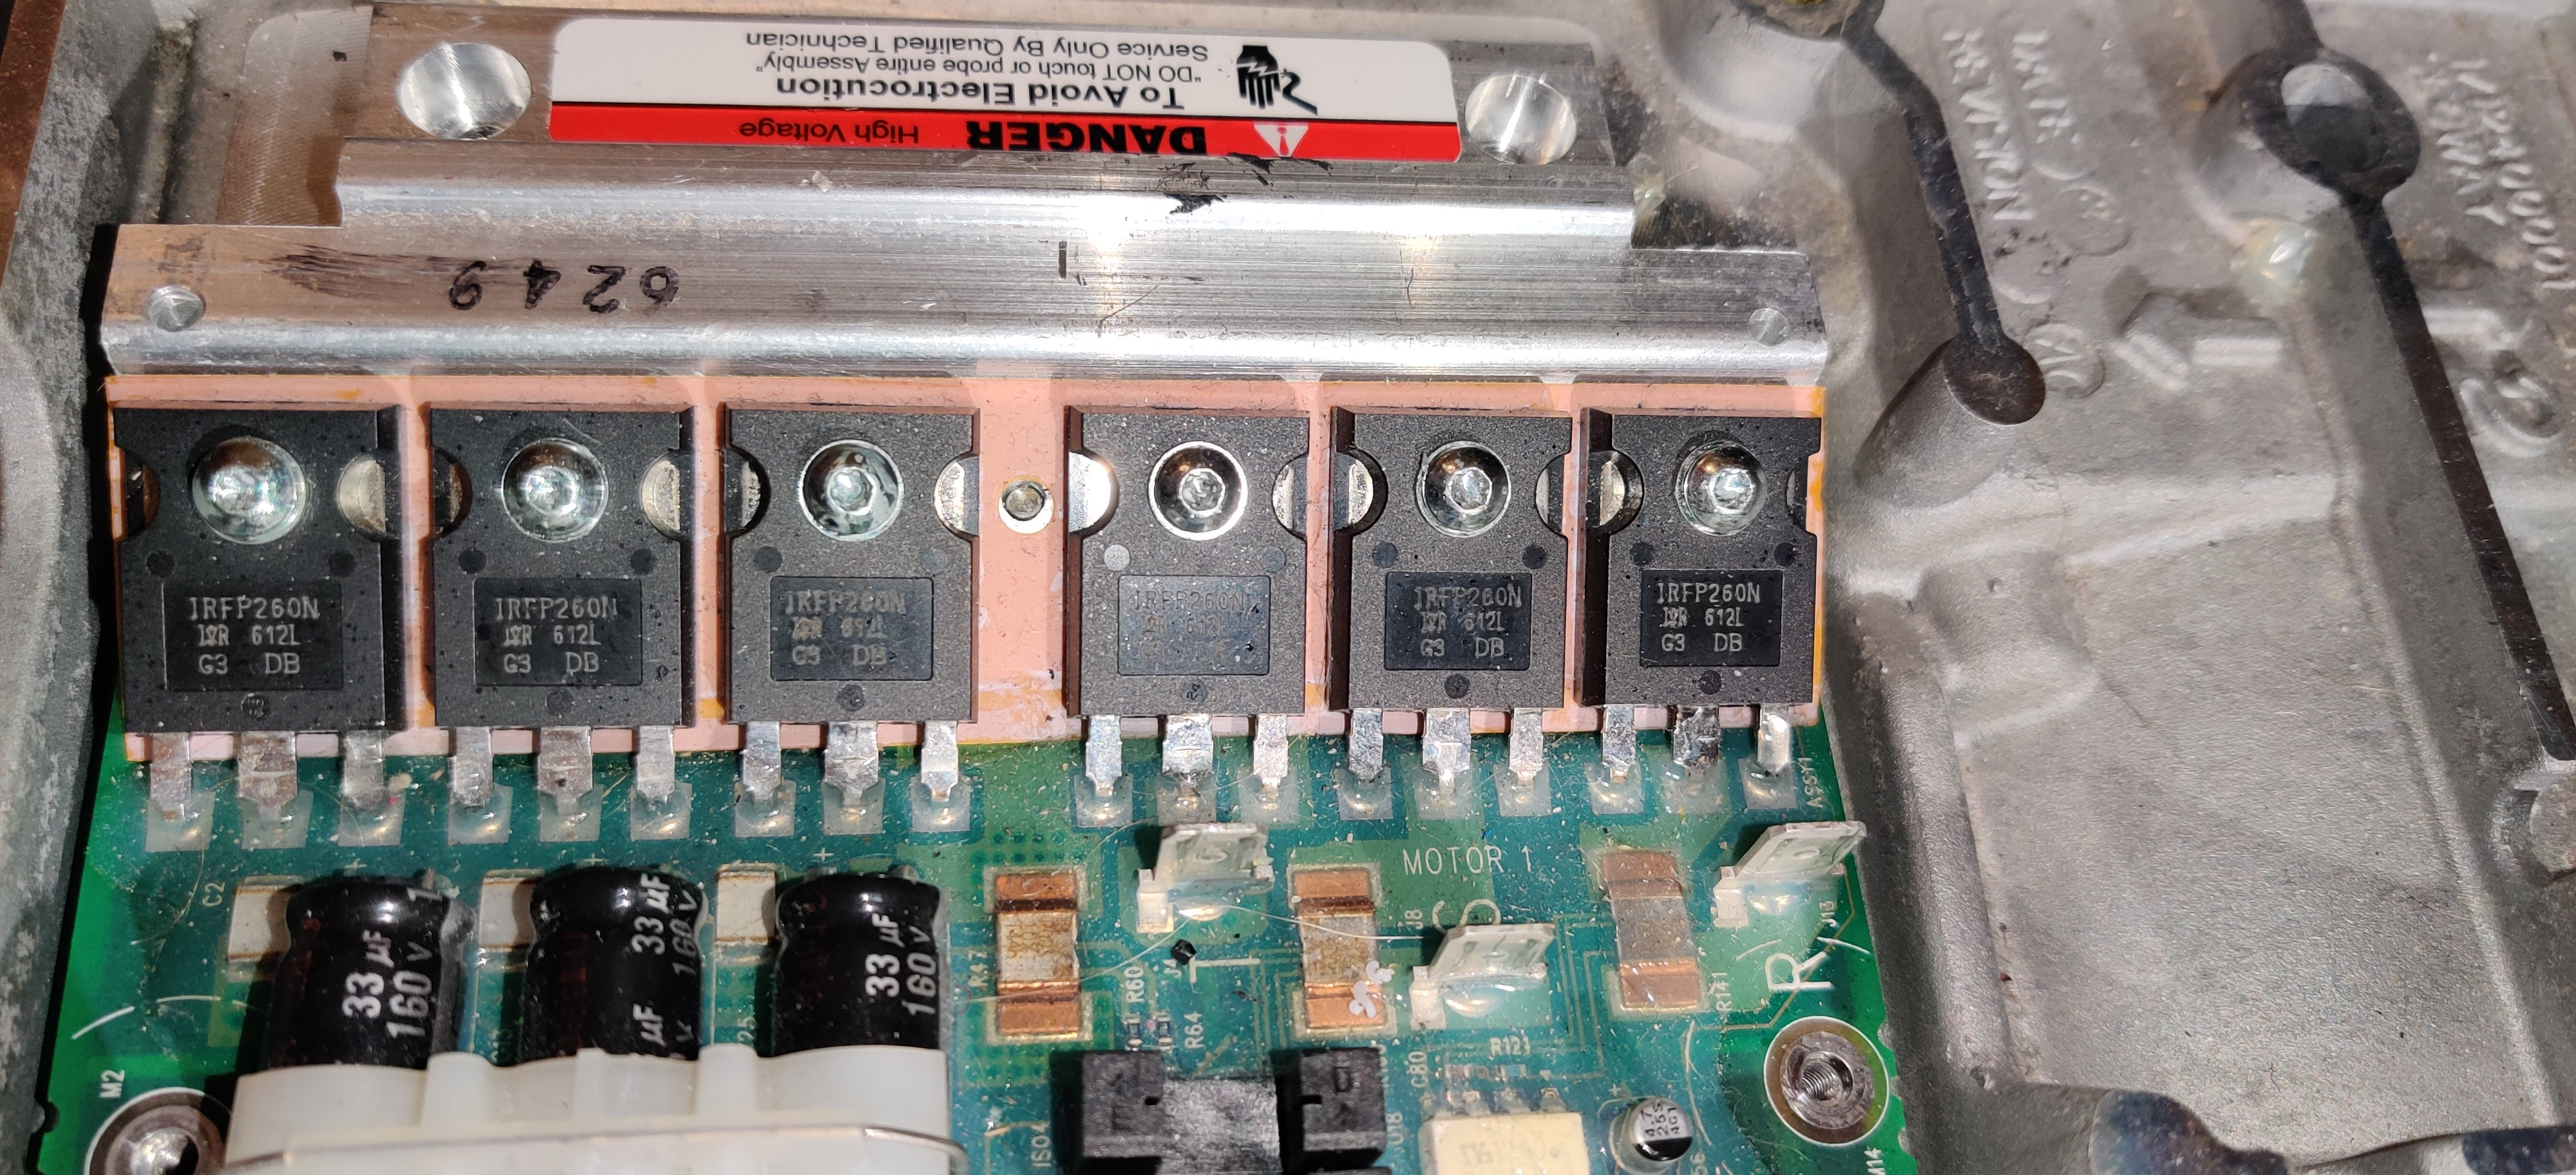
\includegraphics[]{segwayMotorDrivers.jpg}
    \caption{Motor Driver MOSFETS (\ref{Component19}) on one side of a Primary Control Unit}
    \label{fig:segwayMotorDrivers.jpg}
\end{figure}

\subsubsection{Segway Motors \& Motor Driver PCB}

\begin{figure}
    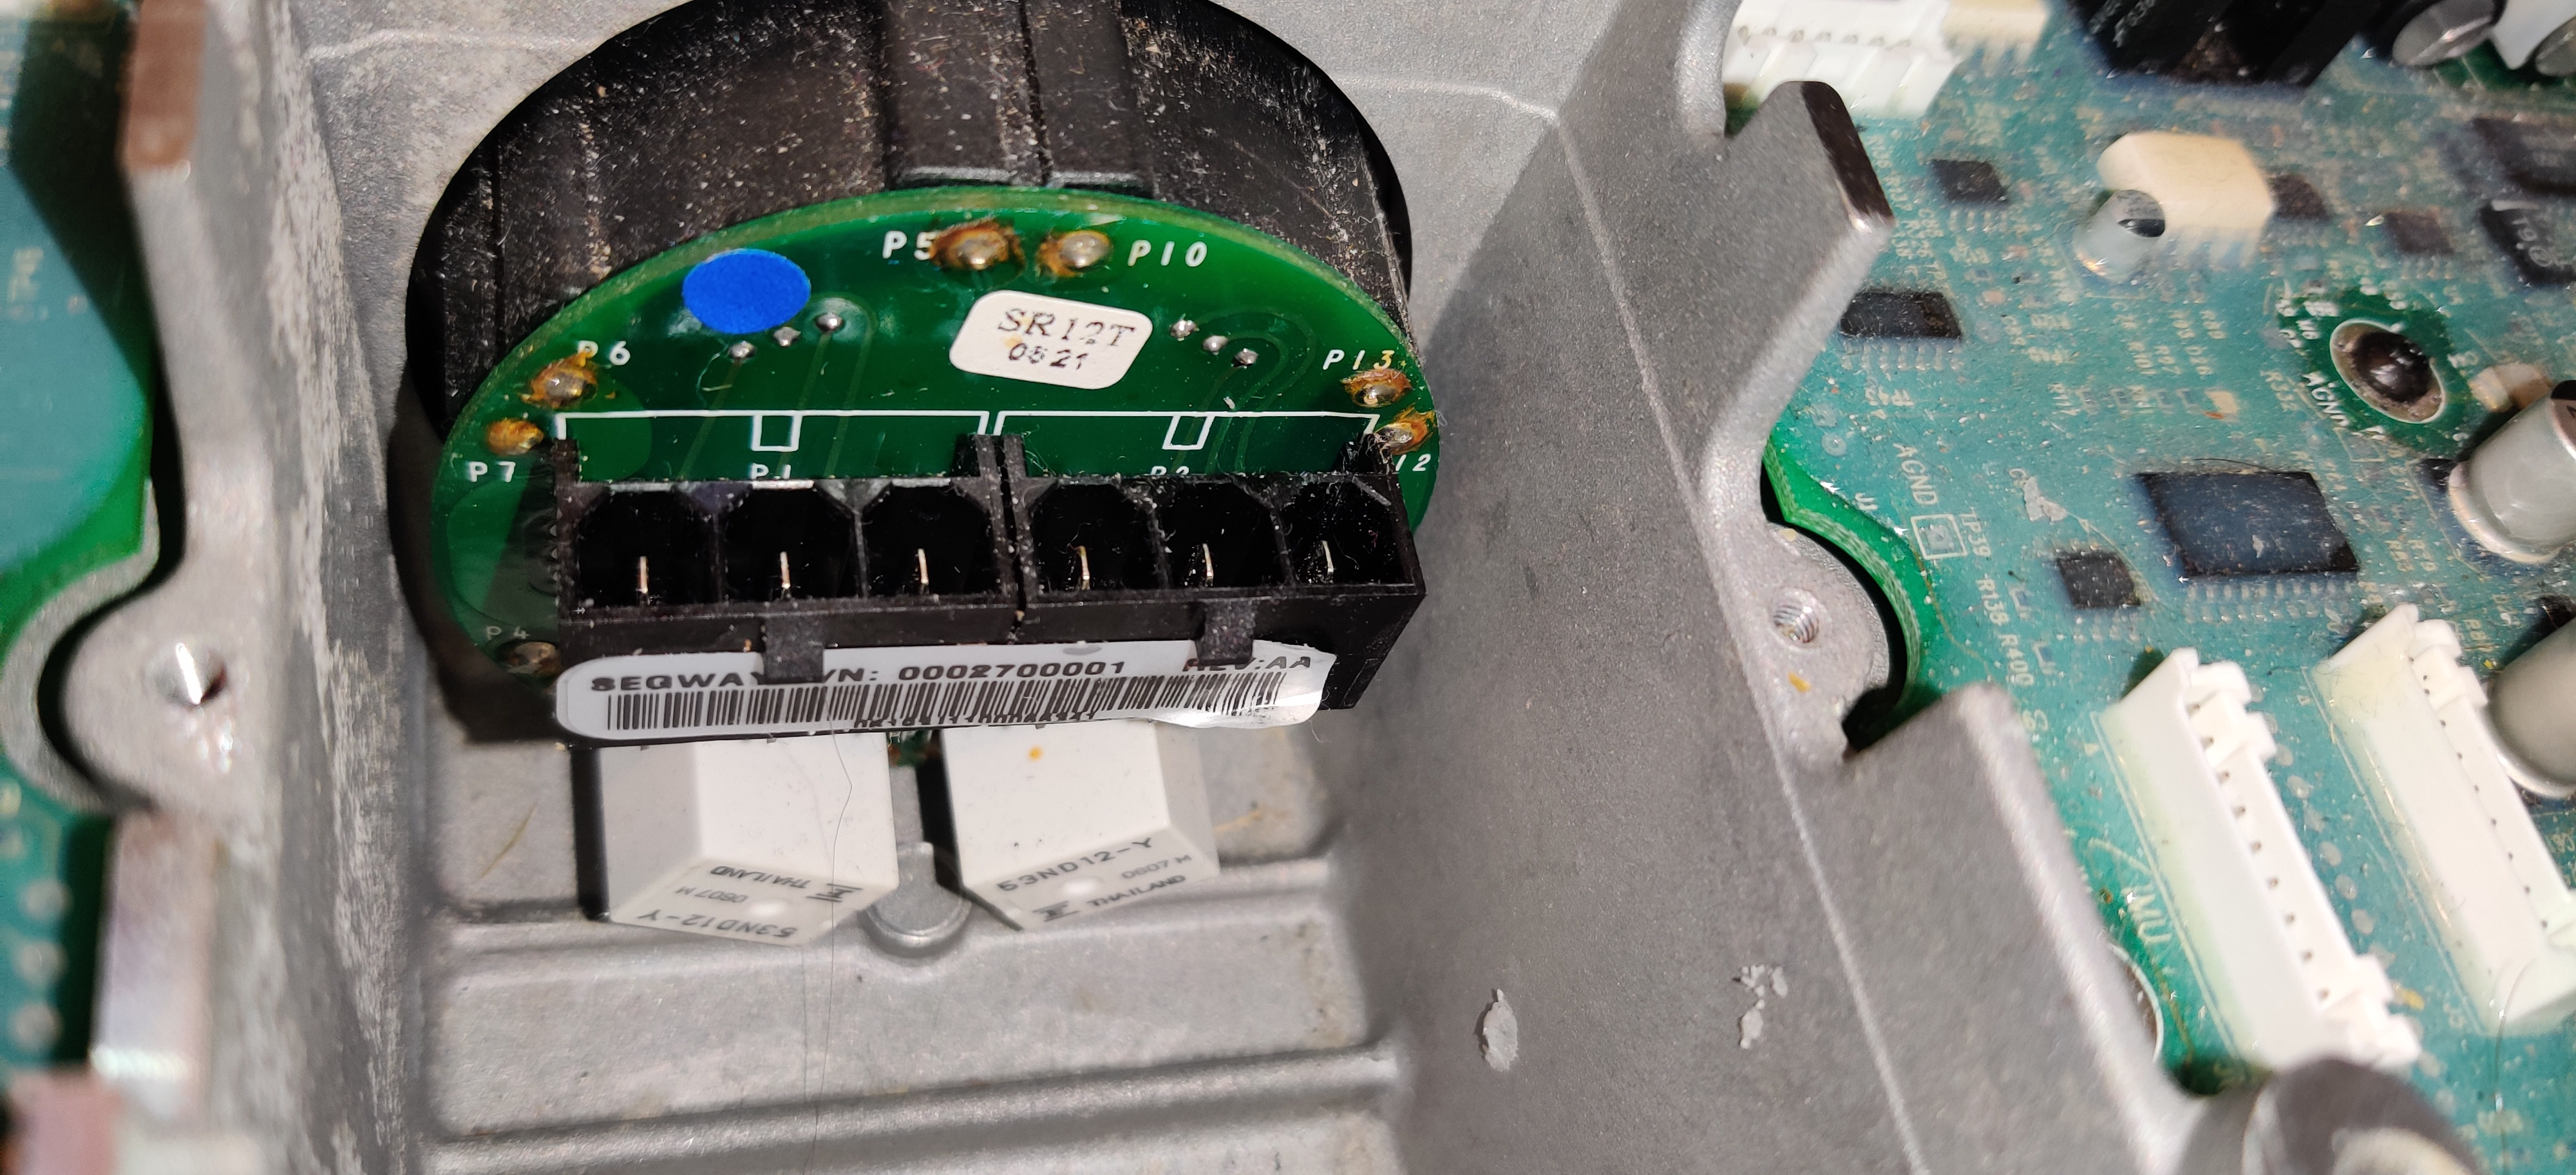
\includegraphics[]{segwayMotorInternal.jpg}
    \caption{Close-up of the PCB Shield on the motor, with dual three-phase inputs (one for each Primary Control Unit)}
    \label{fig:segwayMotorInternal.jpg}
\end{figure}

\begin{figure}
    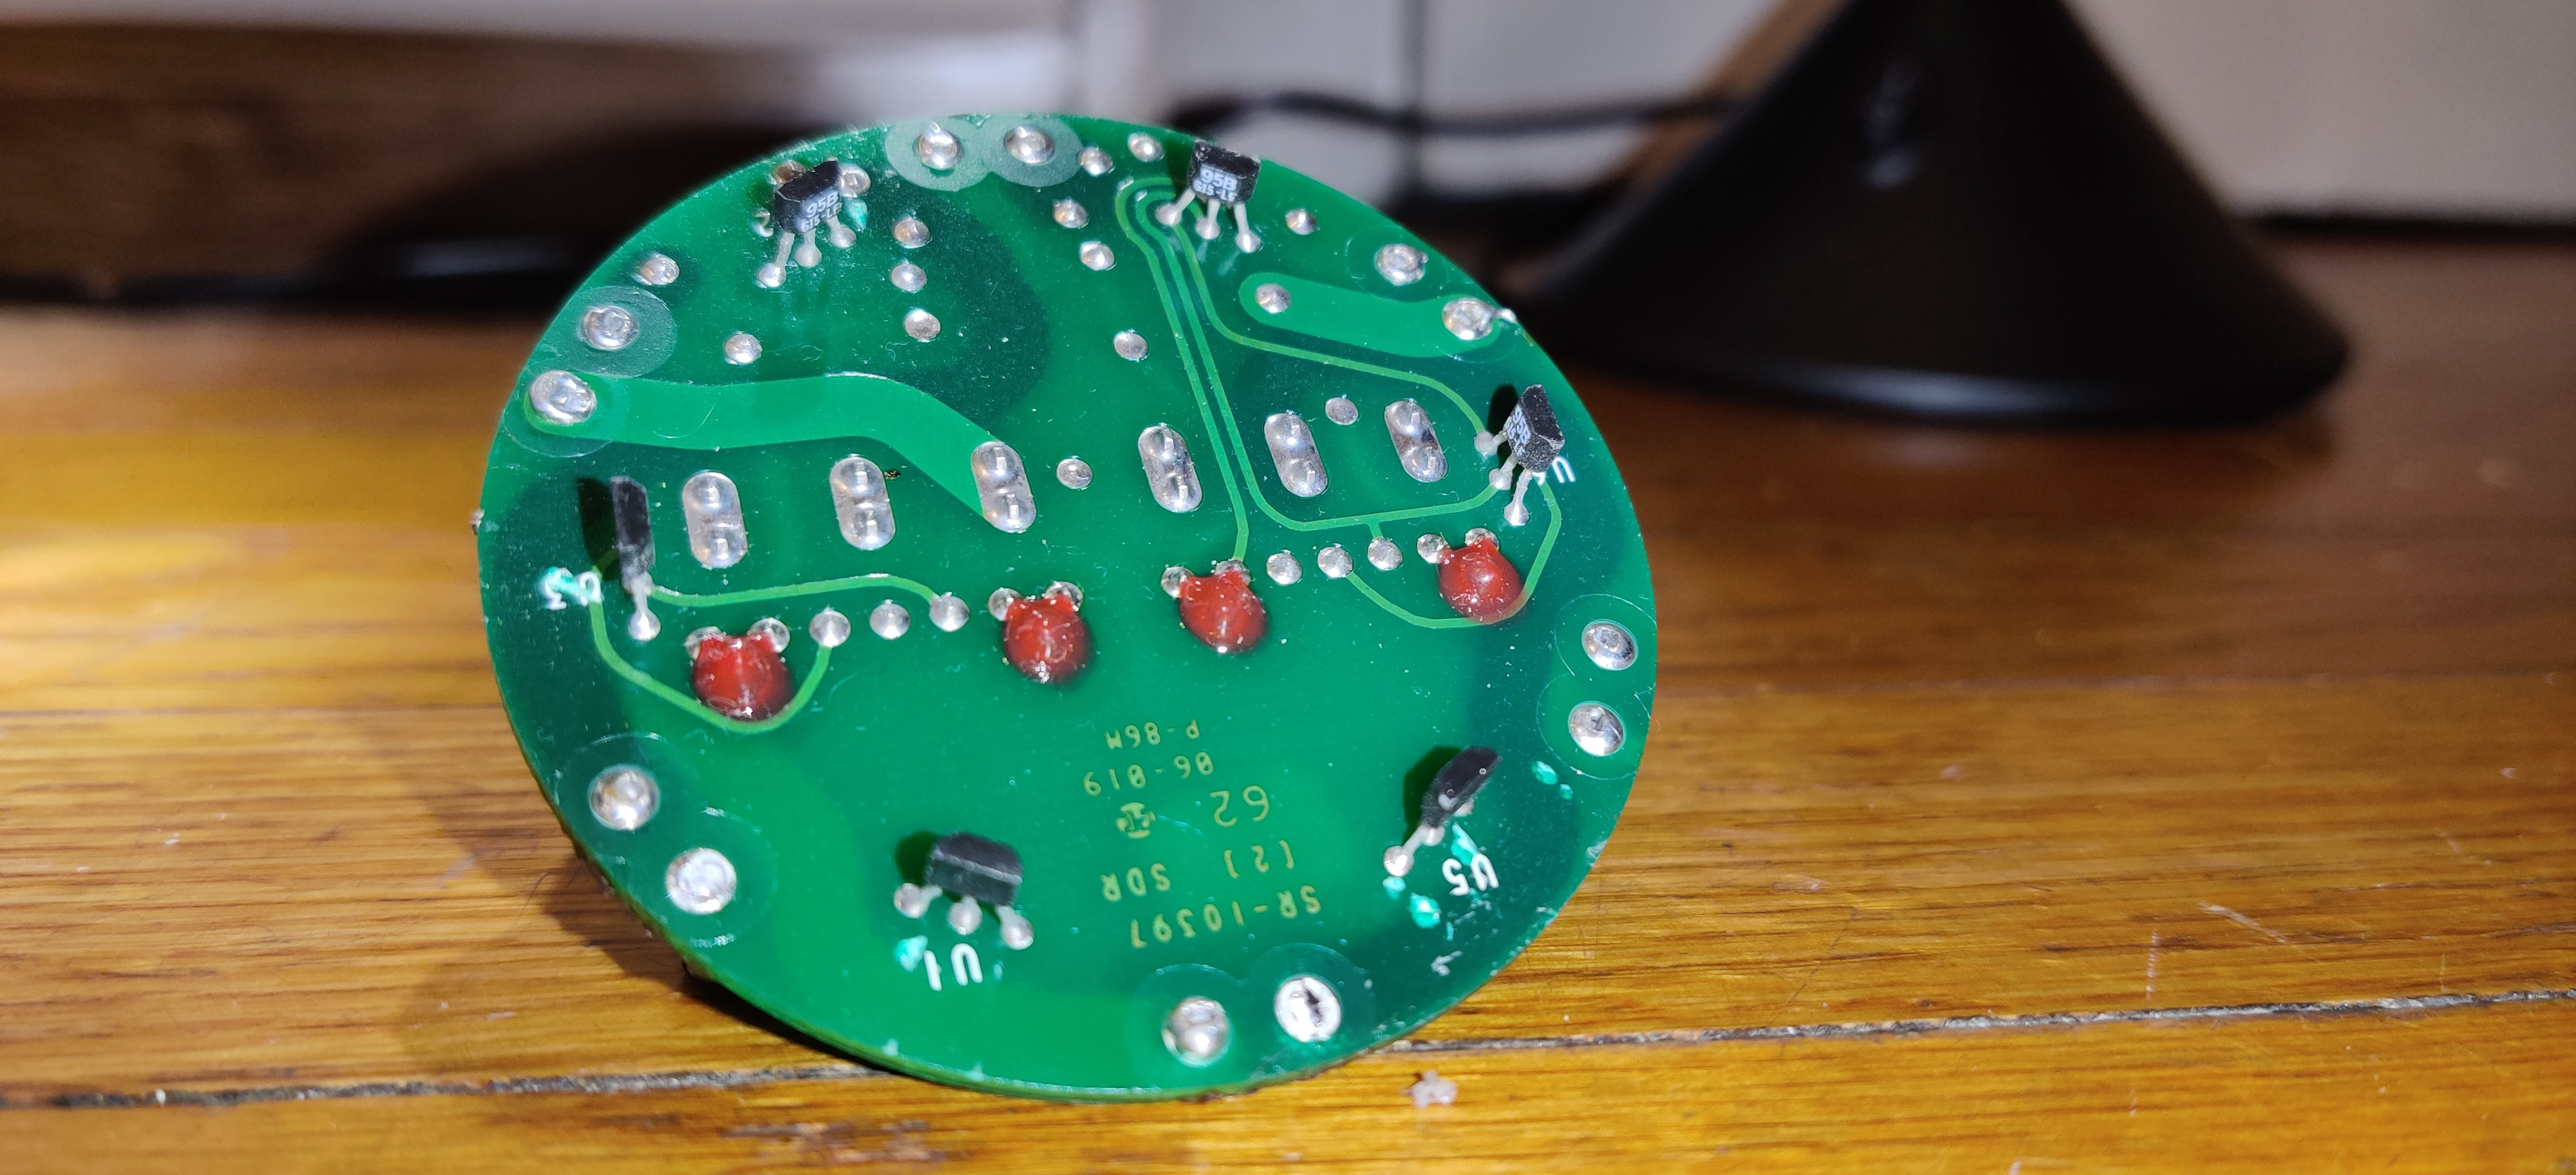
\includegraphics[]{segwayMotorPCBRear.jpg}
    \caption{Rear view of the Motor PCB after removing from the motor, with 6 hall effect sensors, to measure rotor position}
    \label{fig:segwayMotorPCBRear.jpg}
\end{figure}

\subsubsection{Sensing Unit}

\begin{figure}
    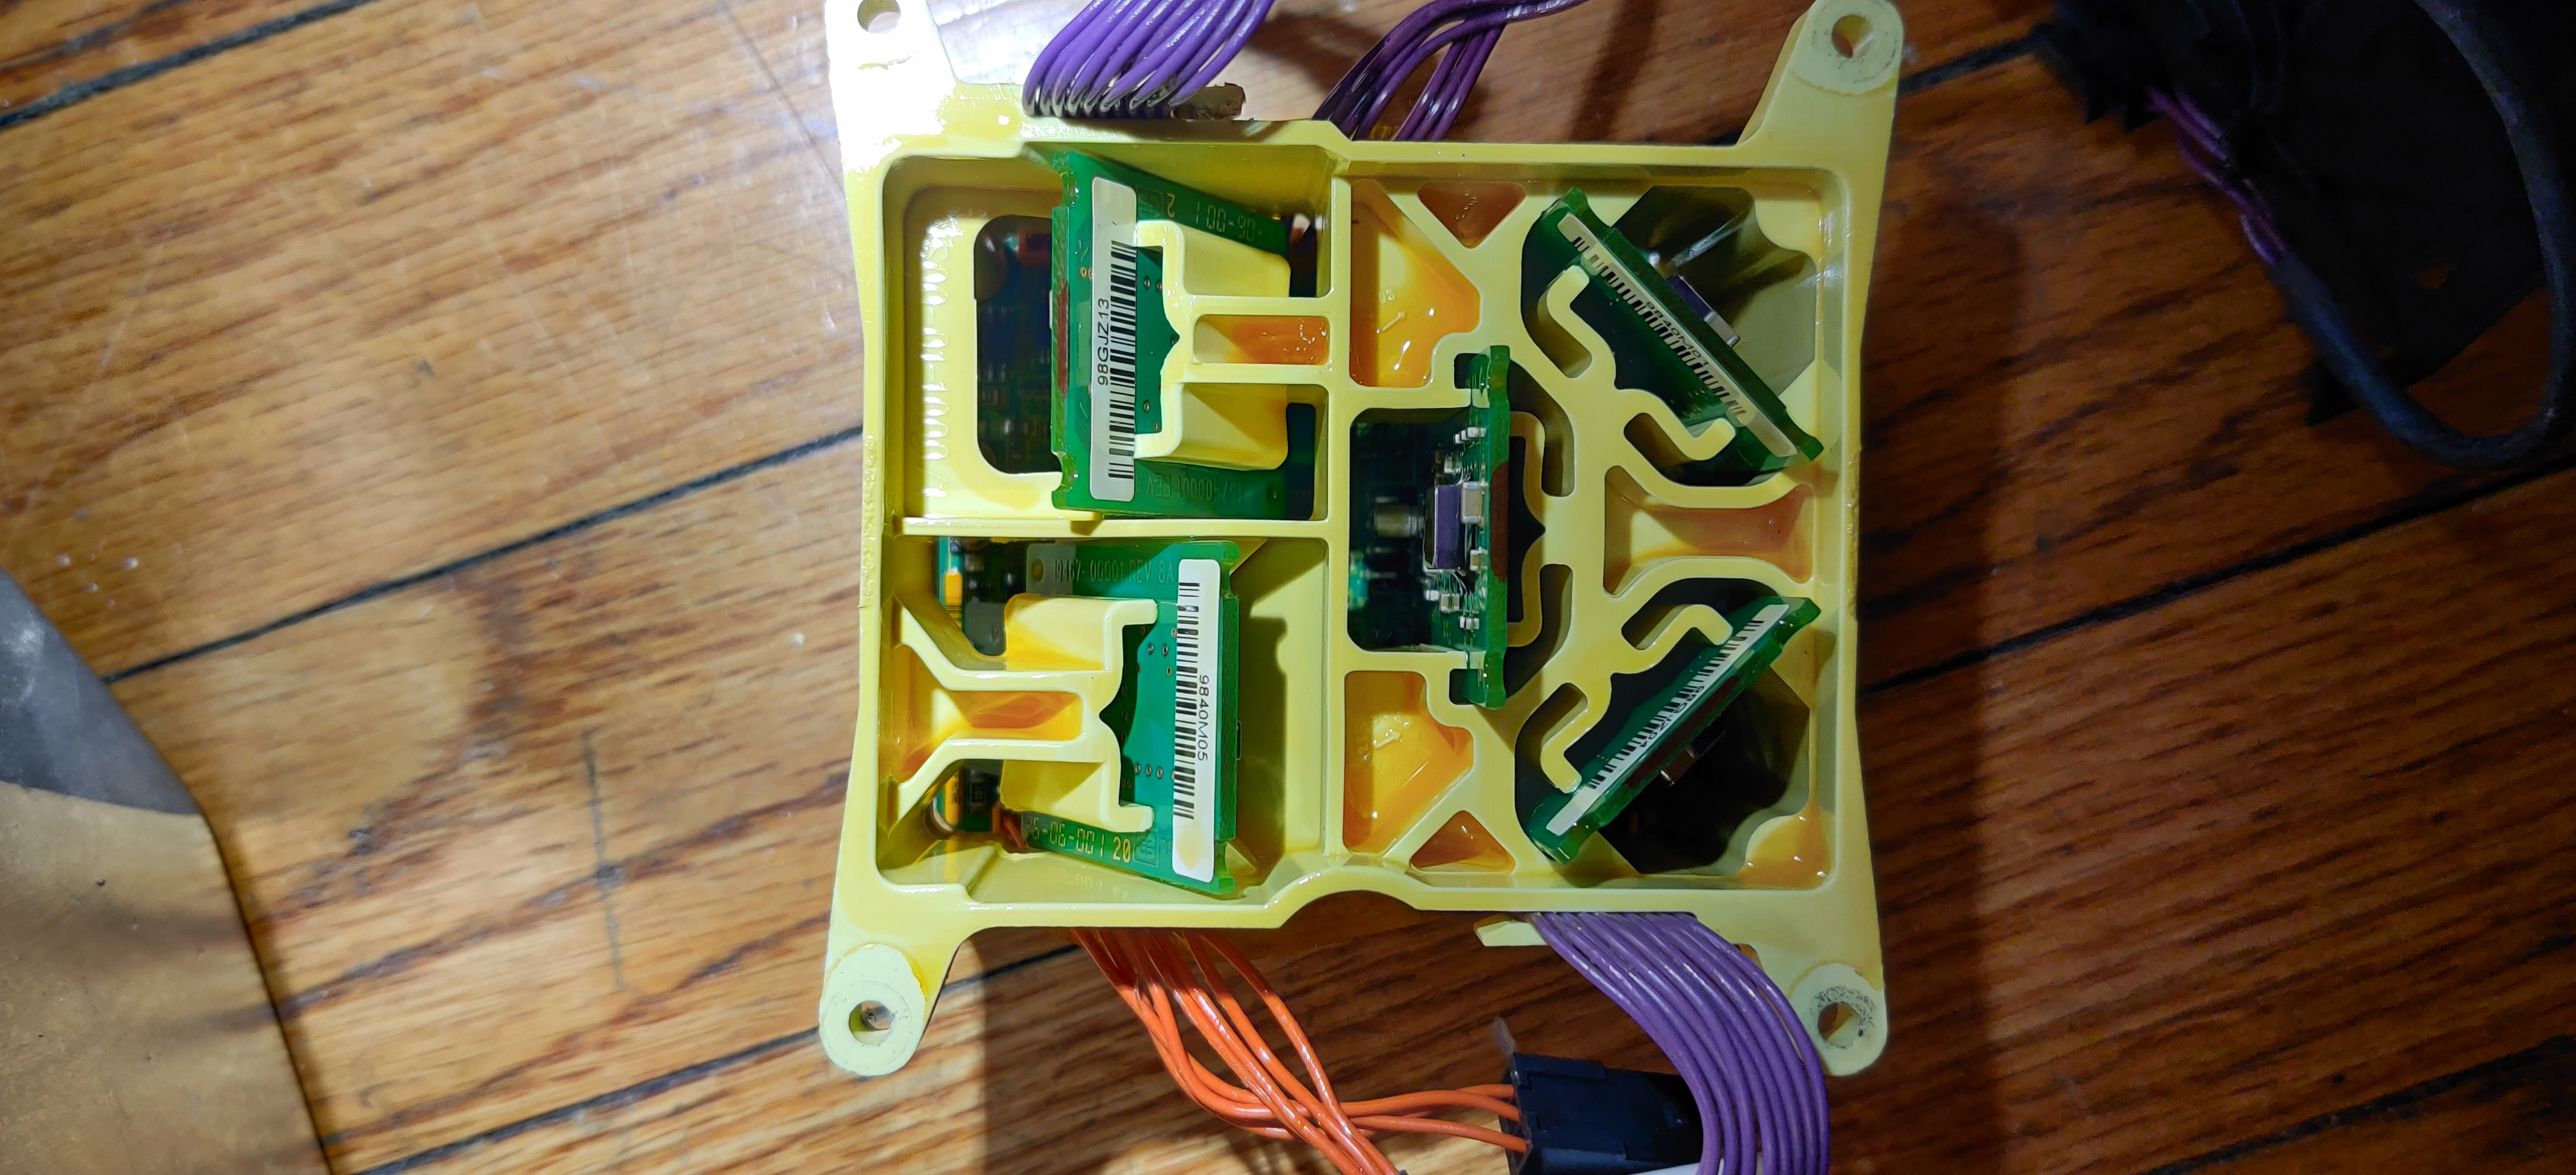
\includegraphics[]{segwayGyroCubeTop.jpg}
    \caption{Top view of the Sensing Unit, with the cast IMU holder keeping the IMUs from moving out of position}
    \label{fig:segwayGyroCubeTop.jpg}
\end{figure}

\begin{figure}
    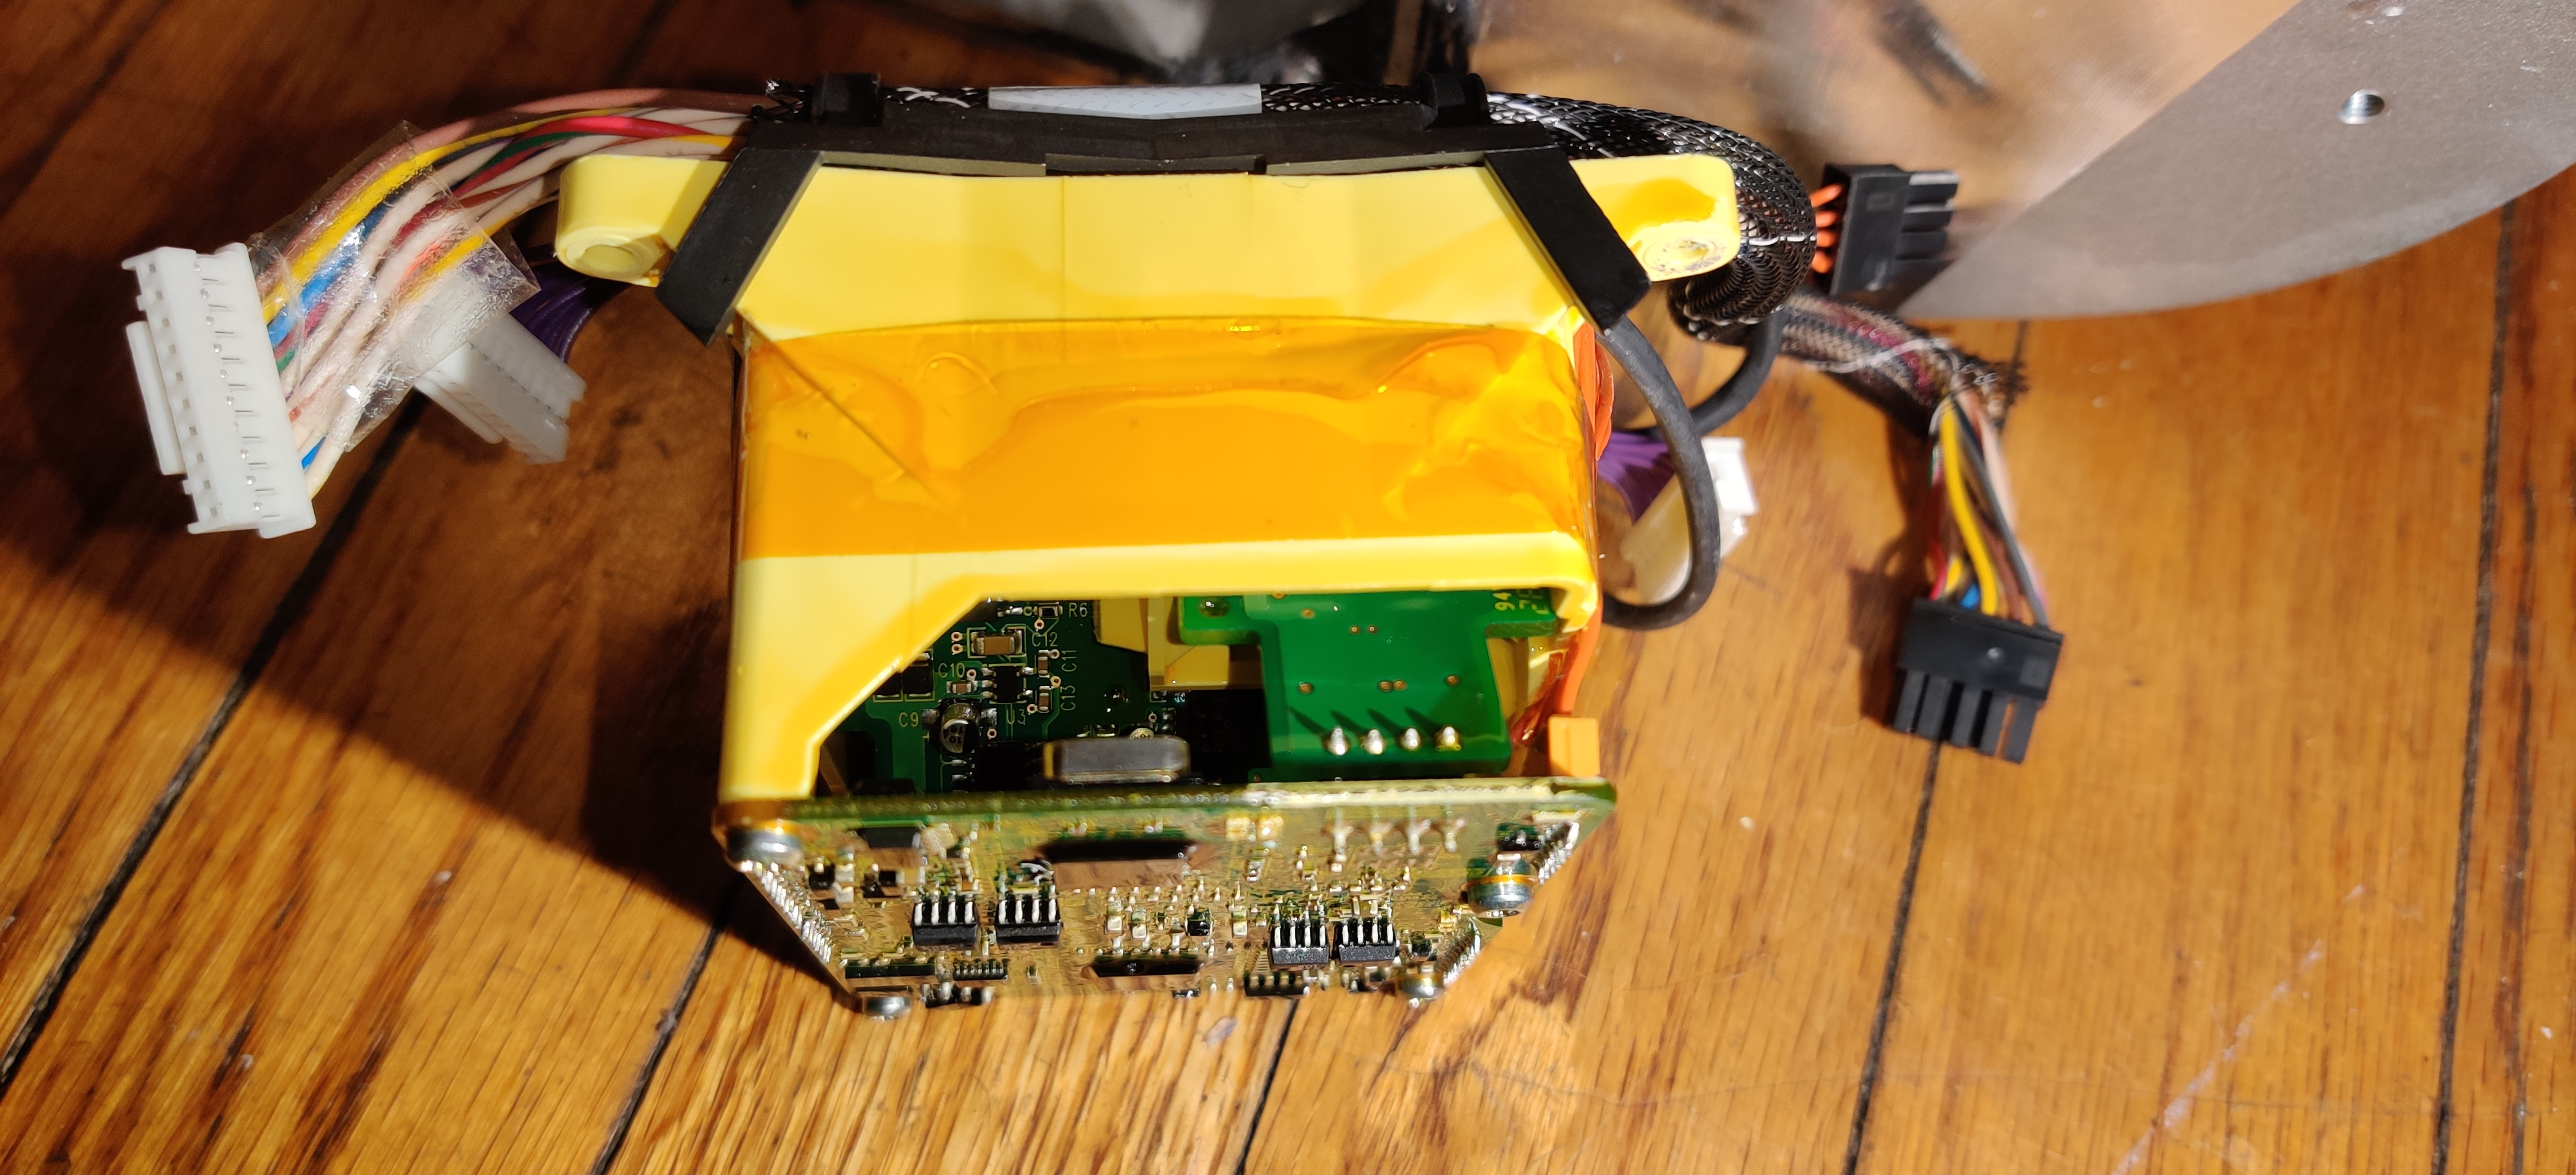
\includegraphics[]{segwayGyroCubeSide.jpg}
    \caption{Side view of the Sensing Unit, with the cast IMU holder attached to the module}
    \label{fig:segwayGyroCubeSide.jpg}
\end{figure}

\begin{figure}
    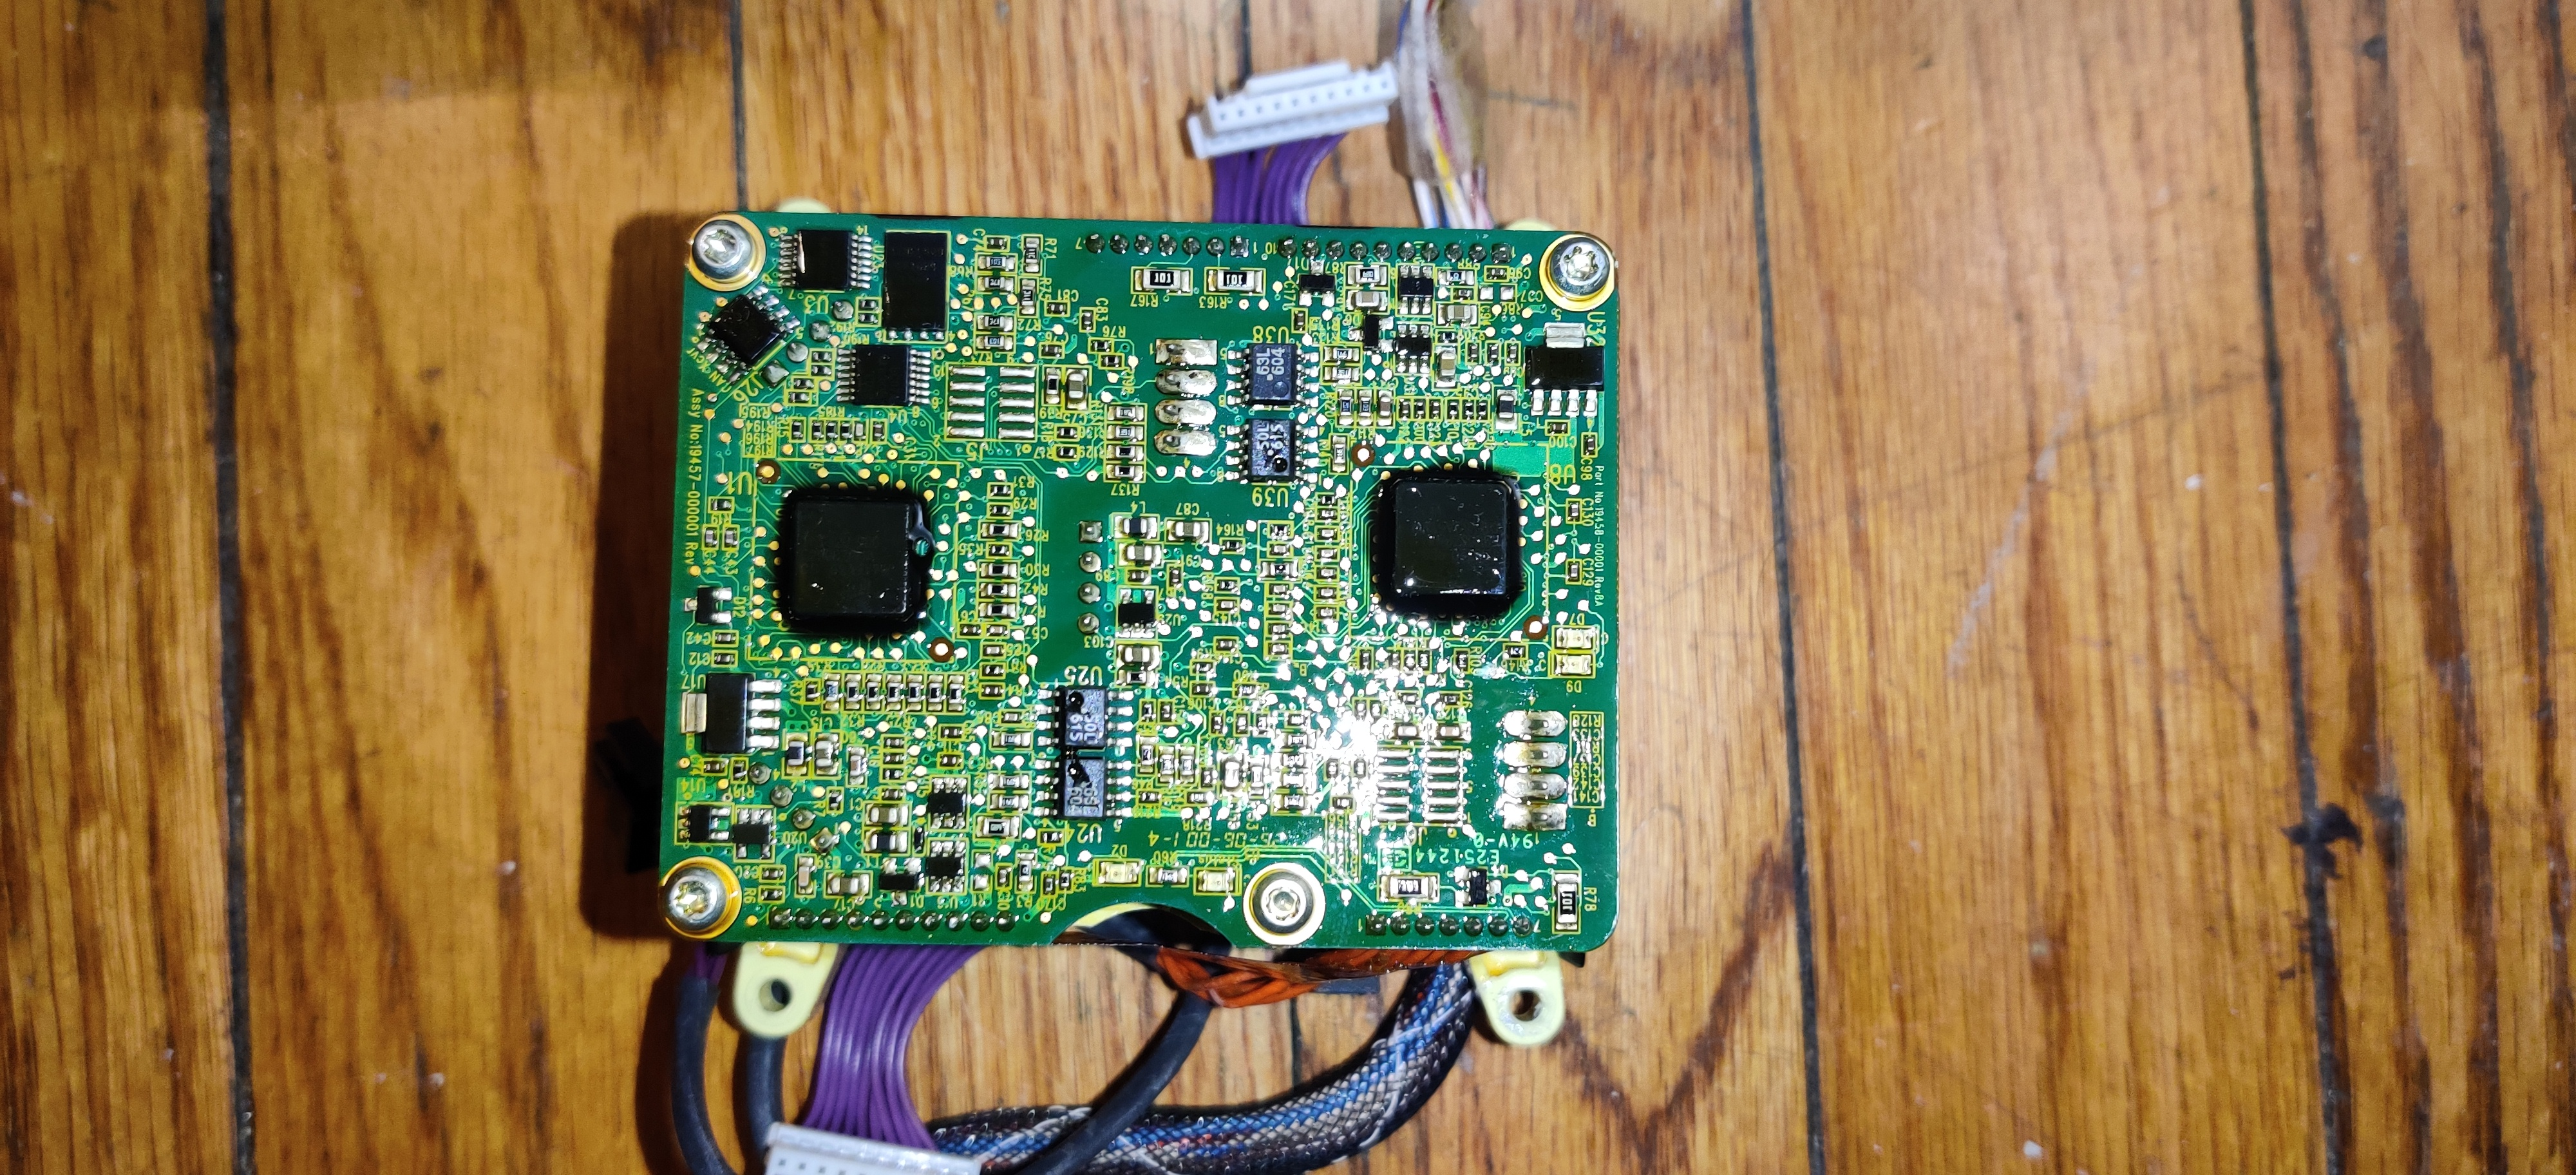
\includegraphics[]{segwayGyroCubeBottom.jpg}
    \caption{Bottom view of the Sensing Unit containing the IMU units, placed on center below the platform}
    \label{fig:segwayGyroCubeBottom.jpg}
\end{figure}

\end{document}
